\documentclass{beamer}
\usetheme{CambridgeUS}
\usecolortheme{seahorse}
\usepackage{comment}
\usepackage{ragged2e}
\usepackage{amsmath}
\usepackage{dcolumn}
\usepackage{booktabs}
\usepackage{pdflscape}
\usepackage{graphicx}
\usepackage{placeins}
\usepackage{dcolumn}
\usepackage{xcolor}
\usepackage{booktabs}
\linespread{1.5}
\usepackage{subcaption}
\usepackage{amsmath}
\usepackage{hyperref}
\usepackage{multirow}
\usepackage{tikz}
\usepackage[title]{appendix}
\usetikzlibrary{decorations.pathreplacing}
\usepackage{appendixnumberbeamer}
\usepackage{booktabs}
\usepackage{tabularx}
\usepackage{ragged2e} 
%\usepackage{xepersian}
%\settextfont{XB Zar}
%\setdigitfont{XB Zar}
\usepackage{array}
\hypersetup{
	colorlinks=true,
	linkcolor=black,
	filecolor=black,      
	urlcolor=black,
	citecolor = blue
}
\setbeamertemplate{itemize items}[square]
%\setbeamercolor{itemize item}{fg=red}  

\setbeamertemplate{itemize subitem}[triangle]
%\setbeamercolor{itemize subitem}{fg=red}
\usepackage[authoryear]{natbib}

\addtobeamertemplate{block begin}{}{\justifying} 
\renewcommand{\today}{\ifcase \month \or January\or February\or March\or %
	April\or May \or June\or July\or August\or September\or October\or November\or %
	December\fi, \number \year} 


\usepackage{array}
\usepackage{booktabs}
\usepackage{caption}


\newcommand{\rowfonttype}{}% Current row font
\newcommand{\rowfont}[1]{% Set current row font
	\gdef\rowfonttype{#1}#1%
}
\newcolumntype{C}{>{\rowfonttype}c}
\newcolumntype{L}{>{\rowfonttype}l}



\AtBeginSection[]
{
	\begin{frame}
		\frametitle{Table of Contents}
		\tableofcontents[currentsection]
	\end{frame}
}

\title[Capital Raise]{Stock market reaction to capital raise announcements:}
\subtitle{Evidence from Tehran Stock Exchange}
\author[Aghajanzadeh, Heidari \&Abedifar]{S.M. Aghajanzadeh \qquad M. Heidari \qquad P. Abedifar }
\institute[]{Tehran Institute for Advanced Studies }
\centering

\begin{document}
	
	{\maketitle}
	
	\section{Data}
	\begin{frame}{Data}
		\begin{itemize}
			\item Data consist of $1290$ capital raise for $448$ companies 
			
			\item Four different sources for capital rising: Cash, Resereves, Cash \& Resereves , and Revaluation \\
			
			\begin{table}[htbp]
				\centering
				\label{t1}
				\resizebox{0.7\textwidth}{!}
				{
					\begin{tabular}{lccccc}
						\hline
						\hline
						& \multicolumn{1}{l}{Cash} & \multicolumn{1}{c}{Resereves} & \multicolumn{1}{c}{Cash \& Resereves} & \multicolumn{1}{c}{Revaluation} &  \multicolumn{1}{c}{Sum} \\
						\hline
						Event & 716   & 358   & 115   & 101   & 1290 \\
						Percent & 55.50 & 27.75 & 8.91  & 7.83  & 100 \\
						\hline\hline
					\end{tabular}
				}
				\label{tab:addlabel}
				
			\end{table}%
			
			
		\end{itemize}
		
	\end{frame}
	
	
	
	
	
	
	\begin{frame}{Data Summary}{Raised Capital for each Firm}
		\begin{figure}
			\centering
			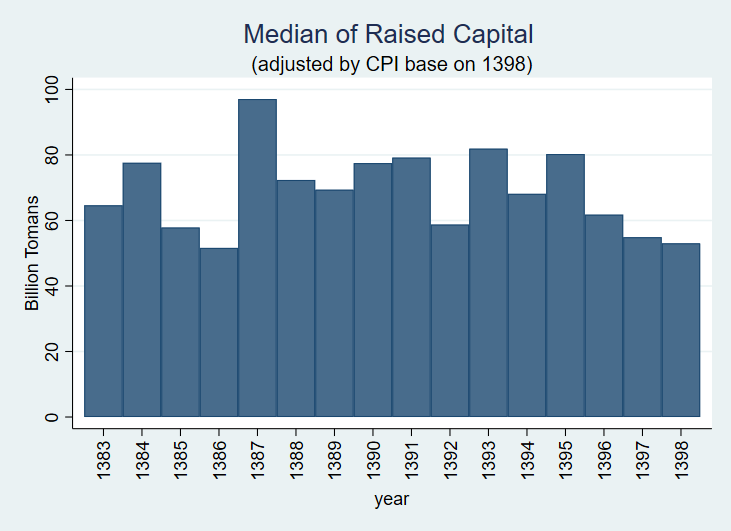
\includegraphics[width=0.7\linewidth]{Output/MedianCapRaiseAdjusted.png}
			\label{fig:mediancapraise}
		\end{figure}
	\end{frame}
	
	\begin{frame}{Data Summary}{Raised Capital for each Firm}
		\begin{figure}
			\centering
			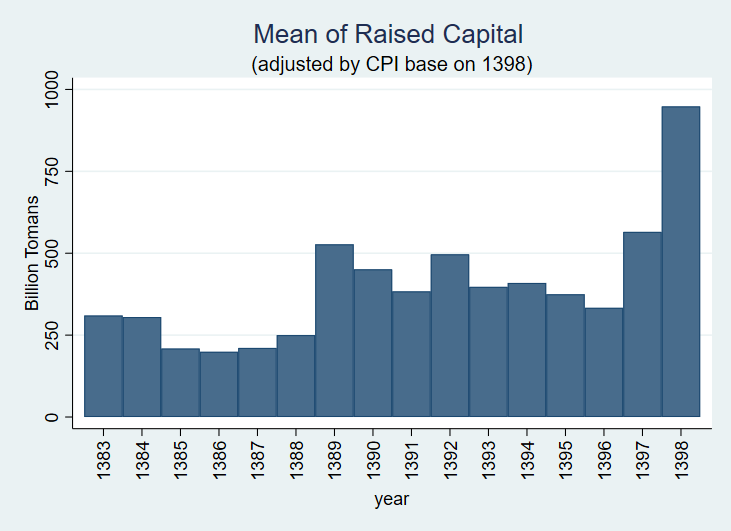
\includegraphics[width=0.7\linewidth]{Output/MeanCapRaiseAdjusted.png}
			\label{fig:meancapraise}
		\end{figure}
	\end{frame}
	
	\begin{frame}{Data Summary}{Adjusted Value of Raised Capital in market}
		\begin{figure}
			\centering
			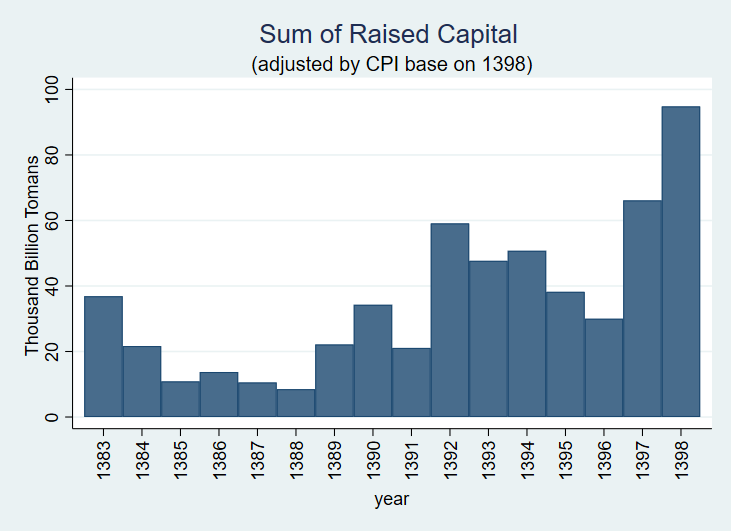
\includegraphics[width=0.7\linewidth]{Output/SumCapRaiseAdjusted.png}
			\label{fig:SumCapRaise}
		\end{figure}
	\end{frame}
	
	\begin{frame}{Data Summary}{Adjusted Value of Raised Capital in market}
		\begin{figure}
			\centering
			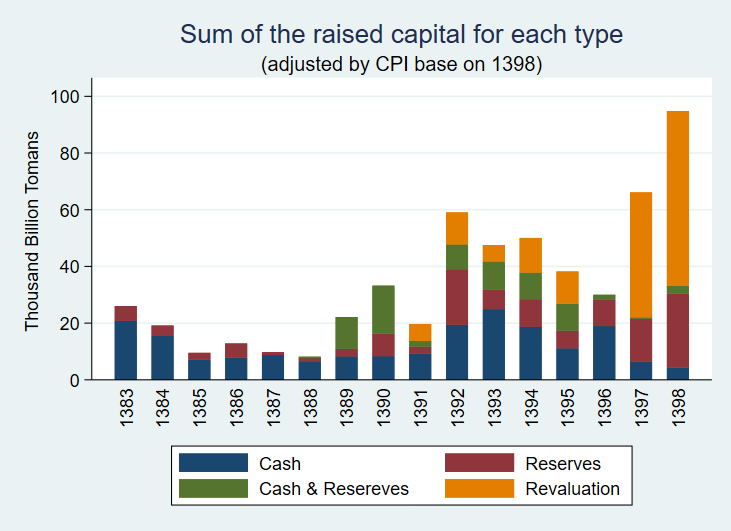
\includegraphics[width=0.7\linewidth]{Output/SumCapRaiseAdjustedEachtype}
			\label{fig:SumCapRaise2}
		\end{figure}
		
	\end{frame}
	
	\begin{frame}{Data Summary}{Percent of Raised Capital for each Firm}
		\begin{figure}
			\centering
			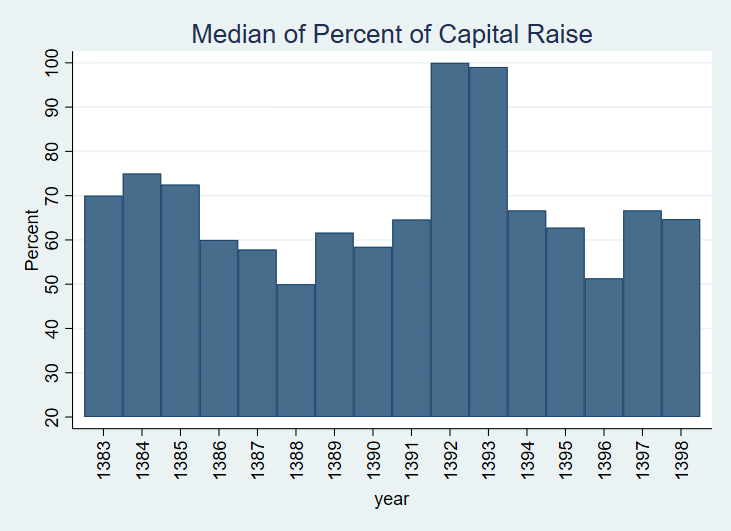
\includegraphics[width=0.7\linewidth]{MedianPercent.png}
			\label{fig:medianpercent}
		\end{figure}
	\end{frame}
	
	\begin{frame}{Data Summary}{Number of Capital Raise}
		\begin{figure}
			\centering
			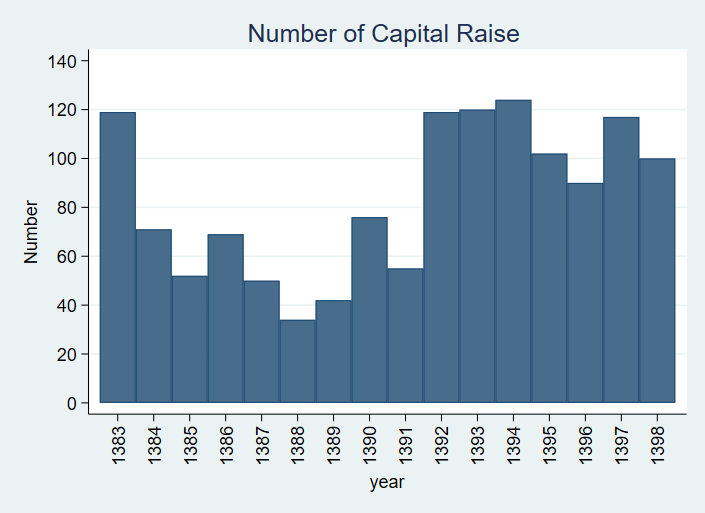
\includegraphics[width=0.7\linewidth]{Number.png}
			\label{fig:number}
		\end{figure}
	\end{frame}
	
	\begin{frame}{Data Summary}{Number of Capital Raise}
		\begin{figure}
			\centering
			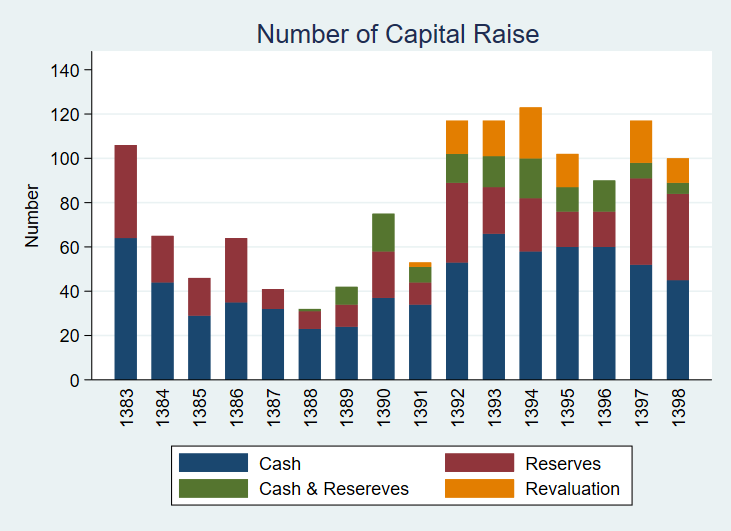
\includegraphics[width=0.7\linewidth]{Number2.png}
			\label{fig:number2}
		\end{figure}
		
	\end{frame}
	%\begin{frame}{Number of Capital Raise}
	%\begin{figure}
	%\centering
	%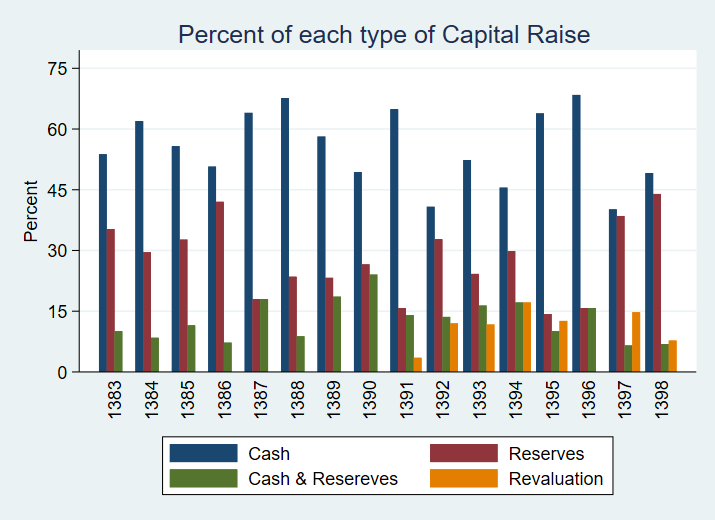
\includegraphics[width=0.7\linewidth]{Number3.png}
	%\label{fig:number3}
	%\end{figure}
	%\end{frame}
	
	%\begin{frame}{Number of Capital Raise for each Firm}
	%\begin{figure}
	%\centering
	%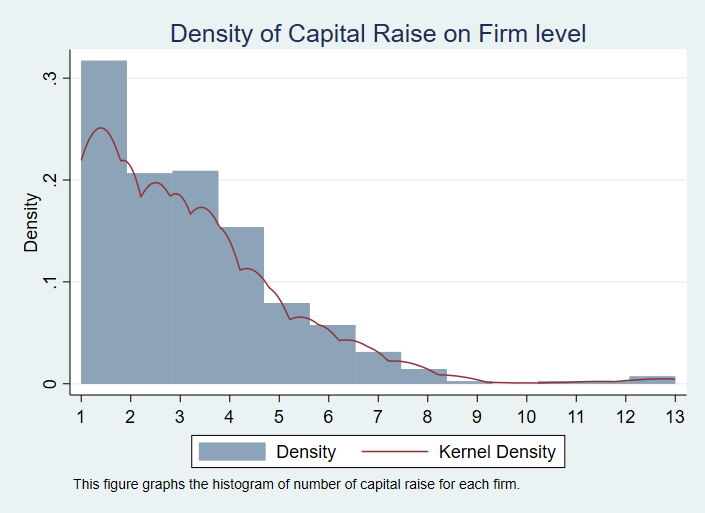
\includegraphics[width=0.7\linewidth]{Hist.png}
	%\label{fig:Hist}
	%\end{figure}
	%\end{frame}
	
	%\begin{frame}{Number of Capital Raise}
	%\begin{figure}
	%\centering
	%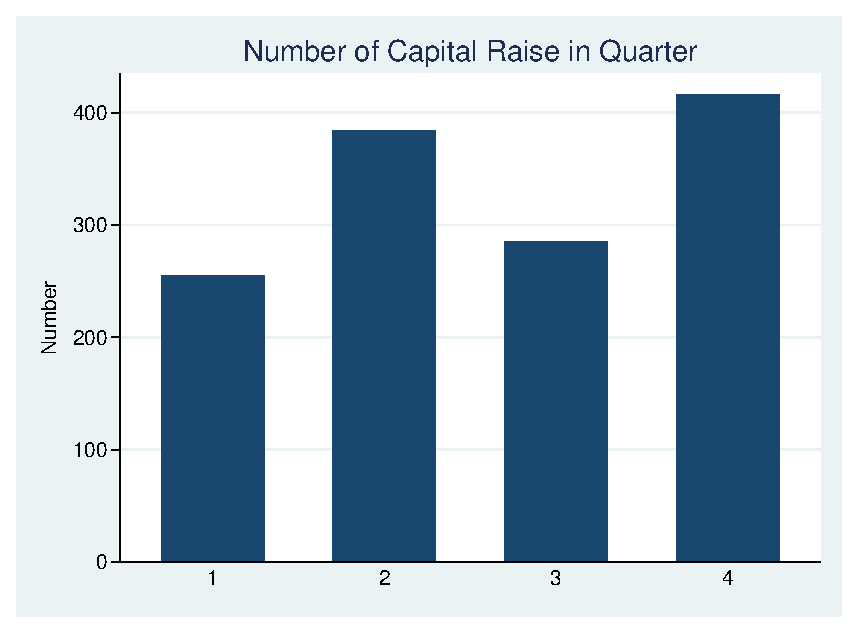
\includegraphics[width=0.7\linewidth]{QNumber}
	%\label{fig:qnumber}
	%\end{figure}
	%\end{frame}
	%
	%\begin{frame}{Number of Capital Raise}
	%\begin{figure}
	%\centering
	%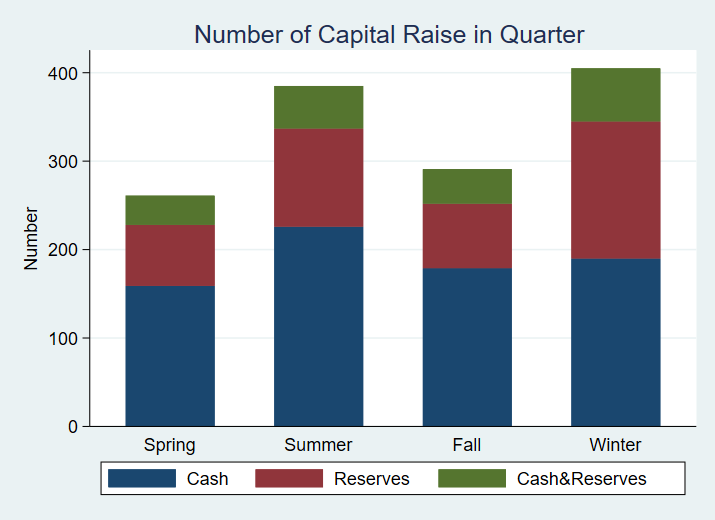
\includegraphics[width=0.7\linewidth]{QNumber2}
	%\label{fig:qnumber2}
	%\end{figure}
	%\end{frame}
	%
	%
	%\begin{frame}{Number of Capital Raise}
	%\begin{figure}
	%\centering
	%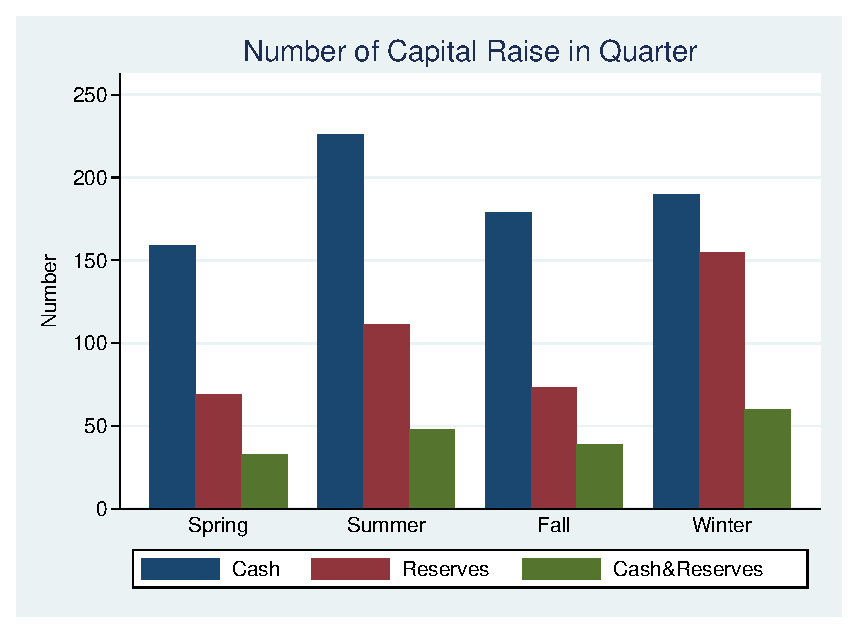
\includegraphics[width=0.7\linewidth]{QNumber3}
	%\label{fig:qnumber3}
	%\end{figure}
	%\end{frame}
	%
	%
	%
	%
	%
	%
	%
	%\begin{frame}{Number of Capital Raise}
	%\begin{figure}
	%\centering
	%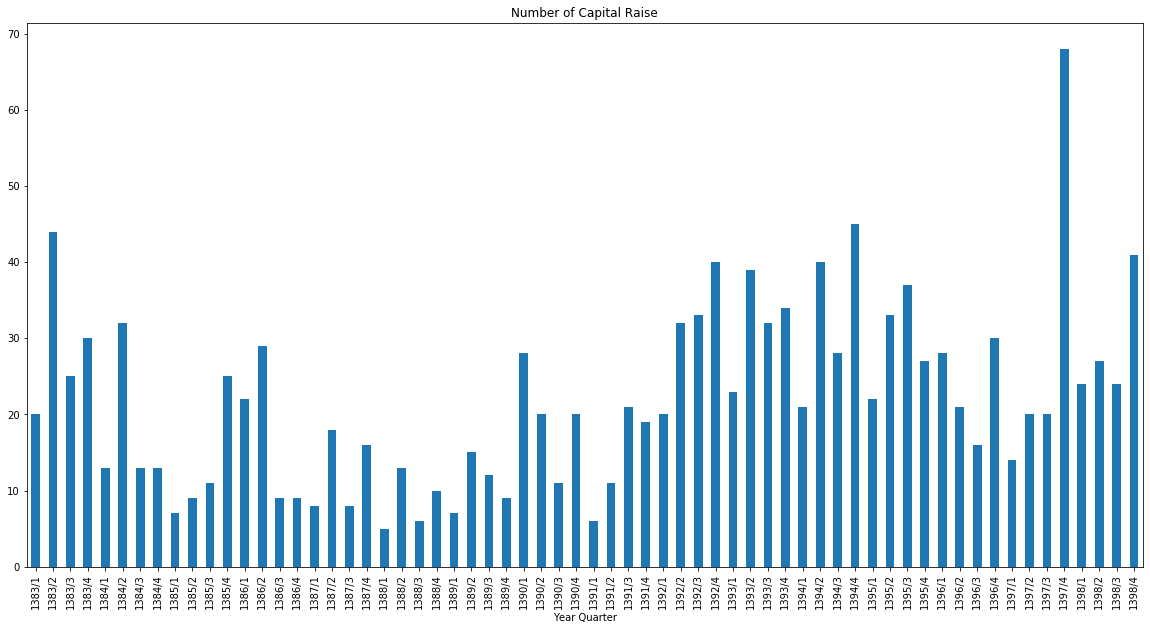
\includegraphics[width=1\linewidth]{Q2Number}
	%\label{fig:q2number}
	%\end{figure}
	%\end{frame}
	%
	%\begin{frame}{Number of Capital Raise}
	%\begin{figure}
	%\centering
	%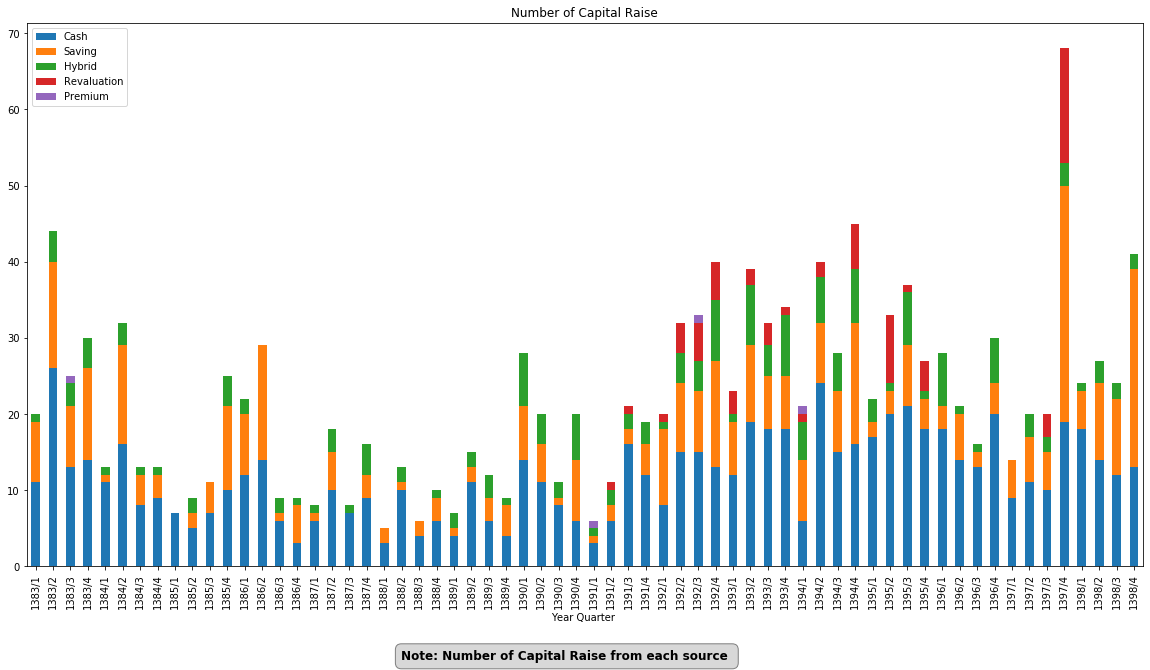
\includegraphics[width=1\linewidth]{Q2Number2}
	%\label{fig:q2number2}
	%\end{figure}
	%\end{frame}
	
	
%	\section{Abnormal Return}
%	
%	\begin{frame}{Abnormal Return}
%		\begin{itemize}
%			\item Abnormal return  is the difference between the observed return and the predicted return
%			\begin{equation*}
%				AR_{i,t} = R_{i,t} - E(R_{i,t}|X_t)
%			\end{equation*}
%			\item Predicted return
%			\begin{itemize}
%				\item Mean-adjusted returns Model (MAR) $ \longrightarrow \bar{R}_i $
%				\item Market-adjusted returns Model (MKAR) $ \longrightarrow {R}_{M,t} $
%				\item Risk-adjusted returns Model (RAR) $ \longrightarrow \alpha_i + \beta_i{R}_{M,t} $
%			\end{itemize}
%		\end{itemize}
%	\end{frame}
%	\begin{frame}{Abnormal Return Calculation}{First Step}
%		
%		
%		%\item  Fama, Fisher, Jensen and Roll (1969)
%		%
%		%\begin{tikzpicture}
%		%	\draw[] (0,0) -- node[below=1mm,pos=0.6,scale=2]{}(10,0)node[right = 4mm]{};
%		%	\draw[] (1,2.5mm)-- +(0,-5.5mm)node[below]{$T_0$};	
%		%	\draw[] (5,2.5mm) -- +(0,-5.5mm)node[below]{$0$};
%		%	\draw[] (9,2.5mm) -- +(0,-5.5mm)node[below]{$T_1$};
%		%	
%		%\draw [decorate,decoration={brace,amplitude=5pt,,raise=2ex}]
%		%  (1,0) -- (9,0) node[midway,yshift=2em]{Estimation Window \& Event Window};
%		%
%		%	\end{tikzpicture}
%		
%		
%		
%		
%		
%		\begin{tikzpicture}
%			\draw[] (0,0) -- node[below=1mm,pos=0.6,scale=2]{}(10,0)node[right = 4mm]{};
%			\draw[] (1,2.5mm) -- +(0,-5.5mm)node[below]{\footnotesize $T_0$};	
%			\draw[] (5,2.5mm) -- +(0,-5.5mm)node[below]{\footnotesize$T_1$};
%			\draw[] (6,2.5mm) -- +(0,-5.5mm)node[below]{\footnotesize$T_1 + 1$};
%			\draw[] (9,2.5mm)  -- +(0,-5.5mm)node[below]{\footnotesize$T_2$};
%			\draw[] (7.5,2.5mm) -- +(0,-5.5mm)node[below]{\footnotesize $0$};
%			
%			\draw [decorate,decoration={brace,amplitude=5pt,mirror,raise=5ex}]
%			(1,0) -- (5,0) node[midway,yshift=-4em]{Estimation window};
%			\draw [decorate,decoration={brace,amplitude=5pt,mirror,raise=5ex}]
%			(6,0) -- (9,0) node[midway,yshift=-4em]{Event window};
%		\end{tikzpicture}
%		\begin{itemize}
%			\item Event windows specifically 3-day, 7-day, and 11-day event periods 
%			\item  Estimation window :  Each event window implies a particular estimation window interval.
%			\scriptsize(For example,
%			3-day event window [-1,+1] is associated with [-122,-2] estimation window)
%			\normalsize
%			\item Fama,Fisher,Jensen, and Roll use Event Window as Estimation window  
%			\tiny[IER-1969-The Adjustment of Stock Prices to New Information]
%		\end{itemize}
%	\end{frame}
%	
%	
%	\begin{frame}{Abnormal Return Calculation}{Second Step}
%		\begin{itemize}
%			\scriptsize
%			\item For each Firm :
%			\begin{equation*}
%				R_{i,t} = \hat{\alpha}_i + \hat{\beta}_i (R_{m,t}) + \boxed{\varepsilon_{i,t}} \rightarrow AR_{i,t}
%			\end{equation*}
%			
%			\item Average abnormal return during period t: 
%			\tiny $ N_t $ is the number of firms in the sample during period t
%			\scriptsize
%			\begin{equation*}
%				AAR_t = \sum_{i=1}^{N_t} \frac{AR_{it}}{N_t}
%			\end{equation*}
%			\item Cumulative Abnormal Returns
%			\begin{equation*}
%				CAR_t(t_1,t_2) = \sum_{t=t_1}^{t_2} {AR_{it}}
%			\end{equation*}
%			\item Cumulative Average Abnormal Return from period $ t_1 $ to period $ t_2 $
%			\begin{equation*}
%				CAAR_{t_1,t_2} = \sum_{i=t_1}^{t_2} CAR_i(t_1,t_2)
%			\end{equation*}
%		\end{itemize}
%	\end{frame}
%	
%	
%	\begin{frame}{Abnormal Return Calculation}{Cross-Sectional Test (Test $ AAR=0 $)}
%		
%		
%		\begin{itemize}
%			\item Hypothesis is  $\left\{\begin{array}{c c }
%				H_0: & AAR=0\\
%				H_1: & AAR\neq 0
%			\end{array}\right.
%			$\\
%			\item[]
%			\item The t-statistics for this test is 
%			\begin{itemize}
%				\item 
%				$
%				t_{AAR} = \sqrt{N}\frac{AAR}{S_{AAR}}
%				$
%				\item 
%				$
%				S^2_{AAR} = \frac{1}{N-1}\sum_{i = 1}^{N}(AR_i - {AAR})^2
%				$
%			\end{itemize}
%		\end{itemize}
%		
%		
%		
%	\end{frame}
%	
%	
%	\begin{frame}{Abnormal Return Calculation}{Cross-Sectional Test (Test $ CAAR=0 $ )}
%		
%		\begin{itemize}
%			\item Hypothesis is  $\left\{\begin{array}{c c }
%				H_0: & CAAR=0\\
%				H_1: & CAAR\neq 0
%			\end{array}\right.
%			$\\
%			\item[]
%			\item The t-statistics for this test is 
%			\begin{itemize}
%				\item 
%				$
%				t_{CAAR} = \sqrt{N}\frac{CAAR}{S_{CAAR}}
%				$
%				\item 
%				$
%				S^2_{CAAR} = \frac{1}{N-1}\sum_{i = 1}^{N}(CAR_i - {CAAR})^2
%				$
%				\item
%				\scriptsize
%				$ CAR_i = \sum_{i=t_1}^{t_2} AR_{i,t} $ 
%				\normalsize 
%			\end{itemize}
%		\end{itemize}
%		
%	\end{frame}
%	
%	
%	
	\section{Literature}
		\begin{frame}{Individual investors}
		\begin{itemize}\tiny
			\item In particular, while institutions are viewed as informed investors, individuals are believed to have psychological biases and are often
			thought of as the proverbial noise traders in the sense of \cite{kyle1985continuous} or \cite{black1986noise}. There is some theoretical models where information flows from investors to managers who make choices that influence the real economy (\cite{FOUCAULT2008146})
				\item  When the information is aggregated through the trades of many individuals the resulting signal may be relatively precise. On the other hand individuals
				may be better positioned to trade aggressively when they are informed.	\cite{kaniel2012individual}
			\item How the
			behavior of different investor clienteles or their interaction in the market affects
			returns?
			\begin{itemize}\tiny
				\item \cite{cohen2002underreacts}:
				\begin{itemize}\tiny
					\item Institutions buy shares from (sell
					shares to) individuals in response to positive (negative) cash-flow news, thus exploiting the
					underreaction phenomenon
					\item When price goes up (down) in the absence of any cash-flow news, institutions sell shares to
					(buy shares from) individuals
				\end{itemize}
				\item Based on the previous day’s stock return, the top performing decile
				of securities is 23.9\% more likely to be bought in net by institutions (and sold
				by individuals) than those in the bottom performance decile. \cite{griffin2003dynamics}
				\item  Individuals tend to buy stocks following declines in the previous month
				and sell following price increases. \cite{kaniel2008individual}
				%				\item  Individual stocks with net buying by retail investors outperform stocks with negative imbalances by approximately 10 bps over the following week. \cite{BOEHMER2021}
				
			\end{itemize}
			
		\end{itemize}
	\end{frame}
	
	
	\begin{frame}{Individuals behavior around events}
		\begin{itemize}\scriptsize
			\item 	\cite{kaniel2012individual} :
			\begin{itemize}\tiny
				\item Intense
				aggregate individual investor buying (selling) predicts large positive (negative) abnormal returns on and after earnings announcement dates
				\item 
				Abnormal returns following the event decomposed  into information and liquidity provision components, and show that about half of the returns can be attributed to private information
			\end{itemize} 
			\item \cite{nguyen2017stock}:
			\begin{itemize}\tiny
				\item There is a evidence consistent with illegal insider trading,
				particularly in firms that were vulnerable to insider manipulation and, therefore, more likely to split
				their stocks. When vulnerable firms’ stocks did split, they provided significant excess short-term
				returns
				
				
				
			\end{itemize}
			\item 
			\begin{itemize}\tiny
				\item  \cite{constantinides1989optimal}
				security issues are used to finance investments and do not necessarily provide signals to the
				market. On the other hand, repurchases do signal information in equilibrium in which part of the
				issue proceeds are used to repurchase
				\item \cite{bond2016buying} undervalued firms that
				would avoid issuing equity to finance positive NPV projects due to SEO underpricing can signal
				their valuation to the market using repurchases. As a result, some firms use repurchases for
				purposes of information signaling and (larger) subsequent SEOs for financing of investment opportunities
			\end{itemize}
		\end{itemize}
	\end{frame}
	
	
	
	\begin{frame}{Information Asymmetric}
		
		\begin{itemize}
			\tiny
			\item \cite{myers1984corporate},
			\cite{dierkens1991information}
			\begin{itemize}
				\tiny
				\item Potential buyers of securities have less information
				about the firms’ prospects than managers, who are likely to issue securities when the
				market price is higher than their value
				\item The greater the level of information asymmetry between insiders and
				investors, the greater the negative price reaction
				\item If new investment opportunities are profitable enough, there is no adverse selection
				problem and, hence, no negative stock price reaction
			\end{itemize}
			
			%\item There are possible signaling tools
			%firms can use to shout out the health condition or riskiness of the firms (dividend, under pricing, warrant issuance, and etc)
			%\begin{itemize}
			%	\tiny
			%	\item  Firms simultaneously declare dividends and announce SEO  to reduce information asymmetry [\cite{john1985dividends},\cite{ambarish1987efficient}]
			%	\item 
			%	\cite{ambarish1987efficient} had also
			%	conducted the empirical research to prove these rational actions.
			%	\item 
			%	The magnitude of negative announcement effect will be less, if
			%	the time difference between the offering announcement and the preceding earnings 	announcement gets closer. \cite{korajczyk1991effect}
			%	\item \cite{lang2000voluntary} found a pattern of firms making more frequent optimistic
			%	disclosures, starting six months before the registration date, to reduce information
			%	asymmetry
			%\end{itemize}
			\item \textbf{Signaling Theory}:‌
			There is asymmetric information between
			corporate insiders and the market for both assets-in-place and growth opportunities. As
			a result, firms issue new equities only when their stocks are overpriced, causing market
			to react negatively to SEO. [\cite{myers1984corporate},\cite{ambarish1987efficient}]
			
			\item \textbf{Agency conflicts} also play an important role in the
			process. Managers, having more information than outsiders, act in the best interest of
			existing shareholders at the expense of the new shareholders by issuing equity when it
			is overvalued. [\cite{myers1984corporate},
			\cite{miller1985dividend},\cite{jensen1986agency}]
			
		\end{itemize}
		
		
	\end{frame}
	
	
	
	\begin{frame}{Capital Structure}
		\begin{itemize}
			\tiny 
			\item \cite{modigliani1958cost} showed that firm’s financing behavior independent
			\item The \textbf{trade-off theory} said that
			firms finance with debt in order to balance the tax advantages of additional debt, or
			marginal tax exceptions, against the costs of possible financial distress. Theoretically, analyses predict that stock price reductions are associated with the source and magnitude
			of financing, i.e. cost of capital, rather than changes in corporate capital structure
			\item Higher debt ratio  demands  risk premium. This risk premium reflects the probability-weighted amount an investor expects to lose in case of the firm failing. In conjunction with the tax shield theory, the firm tries to achieve a static point where the capital structure is at a theoretical cost optimum
			\item Changes in leverage convey a message of insider information about expected changes in future firm performance a higher debt ratio is a binding
			constraint on the firm, and thus signals positive expectations for future cash flows. [\cite{ross1977determination} , \cite{downes1982signaling}] 
			\item  Changes in expected cash flows are positively correlated with changes in optimal leverage levels. Therefore, a decrease in leverage is a negative
			signal to firm value [\cite{deangelo1980optimal},\cite{modigliani1963corporate}]
			\item  Firm’s
			capital structure is one of the factors determining the stock price reaction to external
			financing
			[\cite{dierkens1991information},
			\cite{raymar1993financing}] 
			\cite{cronqvist2005choice}  demonstrated
			statistically that the debt level or risk impacts to SEO choice. The empirical results revealed that there is a negative relationship between leverage and stock price drop after the seasoned equity offerings. [\cite{quyhn2009leverage}]
			\item The marginal increase
			in the level of information asymmetry will be greater for the high-levered firm than the
			low-levered firms 
		\end{itemize}
	\end{frame}
	
	\begin{frame}{Other Theories}
		\begin{itemize}\tiny
			\item Adverse selection: 
			\begin{itemize}
				\tiny
				\item \cite{myers1984corporate} the first to recognize that equity issues to outside investors are associated with an adverse selection problem
				\item \cite{ECKBO1992293}  built on that a rights
				offering with anticipated current shareholder participation (take-up) of less than 100\% is subject to an adverse selection problem
			\end{itemize}
			\item  Downward Sloping Demand Curve and Price Pressure
			Effect
			\item  Pecking Order Theory:
			\begin{itemize}
				\tiny \item  Managers finance
				the needed capital with respect to the order:\begin{enumerate}\tiny
					\item use internally generated cash, \item issue
					debt \item issue hybrid securities \item issue equity
				\end{enumerate}
			\end{itemize}
%			\item Certification Hypothesis:
%			\begin{itemize}\tiny
%				\item Low discounts imply a
%				high offer price, resulting in a high announcement return. It predicts a negative
%				relationship between the announcement return and the offer price’s discount below the
%				market price
%			\end{itemize}
		\end{itemize}
	\end{frame}
	
	
	
	\begin{frame}{Empirical Solutions}
		\begin{itemize}
			\tiny
			\item \cite{loderer1988stock} states that rights offering cannot alone solve the  information asymmetry problem unless the rights offering is fully subscribed. Two additional requirements for eliminating the information asymmetry problem:
			\begin{itemize}\tiny
				\item The life of the information asymmetry is shorter than the period of time
				between announcement and issue date
				\item  the offer price is set on the announcement date
			\end{itemize}
			\item Corporations that  issue seasoned equity offerings are likely to have potential increases in future earnings in order to at least maintain or increase their cash dividends. [\cite{lasfer1997motivation}]
			\begin{itemize}\tiny
				\item Due to unstable dividend policy, the signaling power of a potential increase in future earnings does not exist or is minimal
				for corporations trading in the ISE. [\cite{adaoglu2006market}]
			\end{itemize}
			\item 
			When shareholders approve issuances, average announcement returns are positive. The closer the vote is to the issuance or the greater is the required plurality, the higher
			are the returns for public offers, rights offers, and private placements. When shareholder
			approval is required, rights offers predominate. These findings suggest that agency problems affect equity issuances and challenge existing adverse selection, market timing, and signaling explanations. [\cite{holderness2018equity}]
		\end{itemize}
	\end{frame}
	
	\begin{frame}{SEOs and Ownership Structure}
		\begin{itemize}\scriptsize
			
			\item  Firms with concentrated share ownership, on the
			average level of control more than 61\%, will choose rights issues. when the degree of current-shareholder take-up in the issue is high,
			firms will prefer rights offerings; vice versa, firms are more likely to issue public
			offerings. [\cite{hansen1982direct},\cite{eckbo1992adverse}]
			\item Rational investors consider managers’ fractional
			stock ownership to be a credible signal of firm value. 
			\cite{leland1977informational}  discovered
			that a decrease in managers’ fractional shareholding is a negative signal about firm
			value. Firms with a high insider ownership concentration
			tend to perform better than firms with a low insider ownership concentration. [\cite{limpaphayom2004ownership}]
			\item Most publicly traded companies in Thailand are under the control of founding families
			and management. With this highly concentrated ownership structure, the agency costs
			of external equity is quite significant
		\end{itemize}
	\end{frame}
	

	\begin{frame}{Our path}
		\begin{enumerate}
			\item Decompose abnormal return to liquidity and information
			\item Trading behavior around each type of SEO (Individual buy or sell, herding)
			\item Examine variation in decomposed elements of abnormal return
			\item Insider trading around event for vulnerable firms and invulnerable.
		\end{enumerate}
	\end{frame}
	
	
	%\begin{frame}
	%	\scriptsize
	%	\begin{itemize}
	%		\item Price reaction to equity issue announcements in high equity issue volume (HOT) periods is lower on average than in low equity issue volume (COLD) periods. [\cite{bayless1996there}]
	%		
	%		\item Firms significantly under perform all of benchmarks
	%		over the five years following the equity issues. 
	%		[\cite{jegadeesh2000long}]
	%		\begin{itemize}
	%			\tiny
	%			\item Similar levels of under performance for both small firms and large firms, and both growth firms and value
	%			firms. 
	%			\item Factor-model benchmarks are miss specified
	%		\end{itemize}
	%	\item  Under performance is concentrated primarily in small issuing
	%	firms with low book to market ratios. [\cite{brav2000abnormal}]
	%	\item Price reaction to right issues for listed Indian firms is a positive but statistically insignificant.[\cite{marisetty2008price}]
	%	\begin{itemize}
	%		\tiny
	%		\item The price reaction is significantly more negative for firms with a family group affiliation
	%		compared to firms with no family group affiliation
	%	\end{itemize}
	%	\item When shareholders approve issuances, average announcement returns are positive \tiny[\cite{holderness2018equity}]
	%	\begin{itemize}
	%		\tiny
	%		\item  Agency problems affect equity issuances and challenge existing adverse selection, market timing, and
	%		signaling explanations.
	%	\end{itemize}
	%	\end{itemize}
	%	
	%\end{frame}
	\normalsize
	%\begin{frame}{Iran}
	%\begin{figure}
	%\centering
	%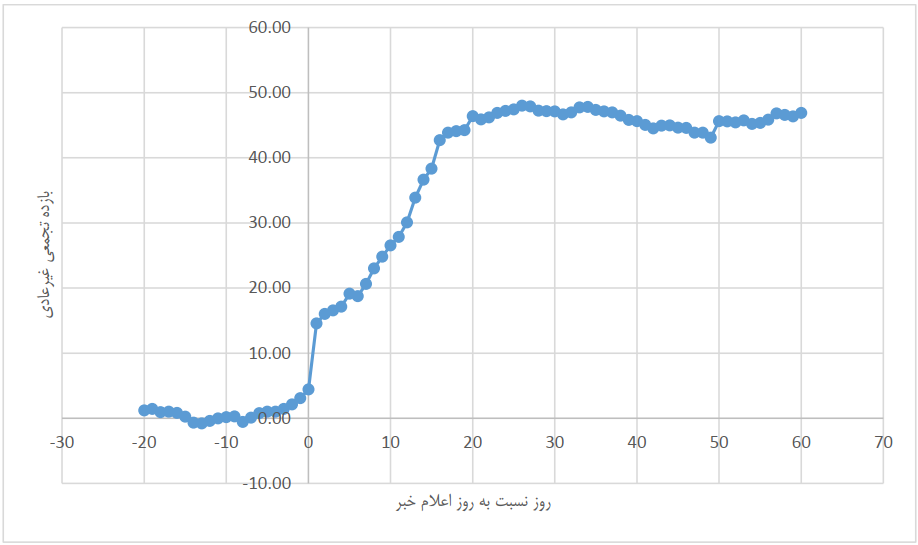
\includegraphics[width=0.65\linewidth]{Soltani}
	%\label{Soltani}
	%\end{figure}
	%\end{frame}
	
	
	\section{Abnormal Return Results}
	\begin{frame}{Abnormal Return}
		
		
		\begin{itemize}
			\item We use the Risk-adjusted returns Model (CAPM) to predict returns.
			\begin{itemize}
				\item We accumulate factors' return in close days for using in the model.
			\end{itemize}
			\item We set estimation and event window as:\\
			\begin{figure}[htbp]
				\centering
				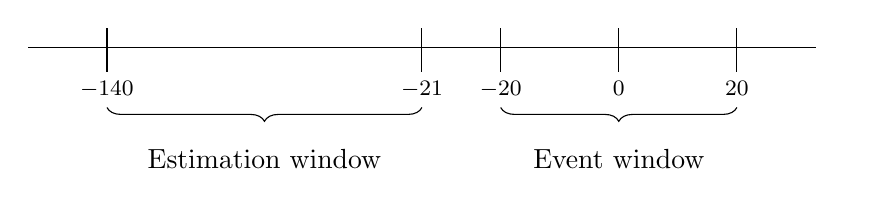
\begin{tikzpicture}
					\draw[] (0,0) -- node[below=1mm,pos=0.6,scale=2]{}(10,0)node[right = 4mm]{};
					\draw[] (1,2.5mm) -- +(0,-5.5mm)node[below]{\footnotesize $-140$};	
					\draw[] (5,2.5mm) -- +(0,-5.5mm)node[below]{\footnotesize$-21$};
					\draw[] (6,2.5mm) -- +(0,-5.5mm)node[below]{\footnotesize$-20$};
					\draw[] (9,2.5mm)  -- +(0,-5.5mm)node[below]{\footnotesize$20$};
					\draw[] (7.5,2.5mm) -- +(0,-5.5mm)node[below]{\footnotesize $0$};
					
					\draw [decorate,decoration={brace,amplitude=5pt,mirror,raise=5ex}]
					(1,0) -- (5,0) node[midway,yshift=-4em]{Estimation window};
					\draw [decorate,decoration={brace,amplitude=5pt,mirror,raise=5ex}]
					(6,0) -- (9,0) node[midway,yshift=-4em]{Event window};
				\end{tikzpicture}
				
			\end{figure}
			
			\item We test whether $ CAAR=0 $ or not
		\end{itemize}
	\end{frame}
	
	\begin{frame}{Estimation Results}
		\begin{table}[htbp]
			\resizebox{0.7\textwidth}{!}{
				\begin{tabular}{lccccccc}
					\hline\hline
					& mean  & std   & min   & 25\%  & 50\%  & 75\%  & max \\
					\hline
					Beta CAPM & 0.80  & 0.84  & -3.62 & 0.28  & 0.69  & 1.18  & 8.81 \\
					Alpha CAPM & 0.16  & 0.39  & -2.42 & -0.05 & 0.09  & 0.28  & 3.60 \\
					\hline
					Beta Market & 0.79  & 0.73  & -5.41 & 0.32  & 0.72  & 1.19  & 4.65 \\
					Beta SMB & 0.14  & 0.28  & -1.14 & -0.01 & 0.07  & 0.22  & 2.33 \\
					Beta HML & 0.02  & 0.27  & -1.43 & -0.09 & 0.02  & 0.14  & 1.65 \\
					Beta WL & 0.06  & 0.26  & -0.71 & -0.07 & 0.03  & 0.15  & 2.10 \\
					Alpha Four & 0.10  & 0.41  & -2.15 & -0.07 & 0.06  & 0.22  & 4.71 \\
					\hline\hline
				\end{tabular}%
			}
		\end{table}
	\end{frame}
	
	\subsection{Abnormal Return}
	\begin{frame}{Abnormal Return}
		\label{abreturn}
		\begin{figure}
			\centering
			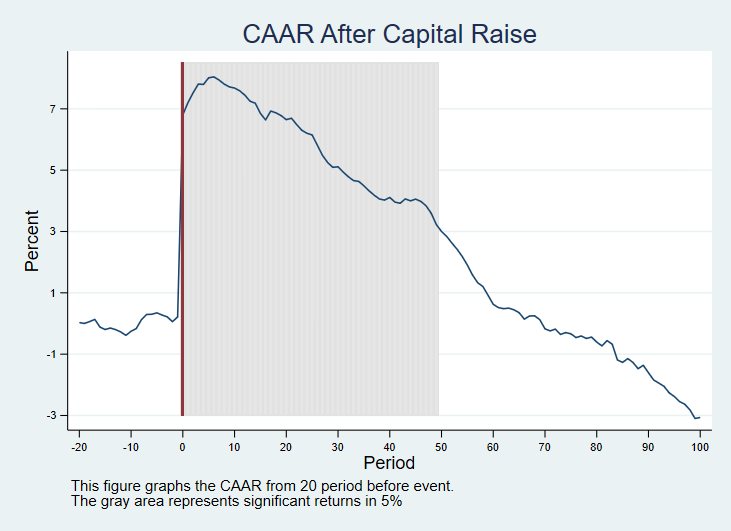
\includegraphics[width=0.7\linewidth]{Output/CAR.png}
			\label{fig:abreturn}
		\end{figure}
		

	\end{frame}
	
%	\begin{frame}
%		% Table generated by Excel2LaTeX from sheet 'Sheet1'
%		
%		
%		\centering
%		\begin{table}[htbp]
%			\centering
%			
%			\captionsetup{labelformat=empty}
%			\caption{\tiny Analysis of abnormal return in days surrounding the capital raise announcements}
%			\centering
%			\resizebox{0.8\textheight}{!}
%			{\tiny
%				\begin{tabular}{cccc|cccc}
%					\hline\hline
%					Period & \multicolumn{1}{c}{AAR} & \multicolumn{1}{c}{CAAR} & \multicolumn{1}{c}{t-stat} & Period & \multicolumn{1}{c}{AAR} & \multicolumn{1}{c}{CAAR} & \multicolumn{1}{c}{t-stat} \\
%					\hline    -20   & 0.06  & 0.06  & 0.45  & 0     & 6.38  & 6.99  & 7.88 \\
%					-19   & -0.06 & 0.00  & -0.02 & 1     & 0.33  & 7.32  & 8.10 \\
%					-18   & -0.03 & -0.03 & -0.15 & 2     & 0.32  & 7.67  & 8.34 \\
%					-17   & 0.08  & 0.05  & 0.23  & 3     & 0.18  & 7.85  & 8.39 \\
%					-16   & -0.16 & -0.10 & -0.42 & 4     & -0.07 & 7.75  & 8.12 \\
%					-15   & -0.06 & -0.16 & -0.59 & 5     & 0.13  & 7.89  & 7.95 \\
%					-14   & 0.04  & -0.13 & -0.43 & 6     & -0.02 & 7.88  & 7.87 \\
%					-13   & 0.05  & -0.08 & -0.24 & 7     & -0.08 & 7.85  & 7.77 \\
%					-12   & -0.08 & -0.16 & -0.47 & 8     & -0.19 & 7.65  & 7.52 \\
%					-11   & -0.09 & -0.25 & -0.68 & 9     & -0.22 & 7.46  & 7.24 \\
%					-10   & 0.18  & -0.06 & -0.17 & 10    & -0.07 & 7.39  & 7.08 \\
%					-9    & 0.18  & 0.12  & 0.29  & 11    & -0.12 & 7.27  & 6.88 \\
%					-8    & 0.29  & 0.40  & 0.93  & 12    & -0.22 & 7.05  & 6.65 \\
%					-7    & 0.16  & 0.59  & 1.30  & 13    & -0.11 & 6.93  & 6.46 \\
%					-6    & -0.01 & 0.58  & 1.23  & 14    & -0.04 & 6.87  & 6.28 \\
%					-5    & 0.41  & 1.00  & 1.80  & 15    & -0.19 & 6.64  & 6.02 \\
%					-4    & -0.09 & 0.91  & 1.59  & 16    & -0.26 & 6.38  & 5.71 \\
%					-3    & -0.11 & 0.81  & 1.37  & 17    & -0.10 & 6.30  & 5.54 \\
%					-2    & -0.22 & 0.58  & 0.95  & 18    & -0.15 & 6.18  & 5.36 \\
%					-1    & 0.04  & 0.62  & 1.01  & 19    & -0.09 & 6.09  & 5.24 \\
%					\hline\hline
%				\end{tabular}%
%			}
%		\end{table}%
%		
%	\end{frame}
%	%
	%\begin{frame}{Abnormal Return}
	%\begin{figure}
	%\centering
	%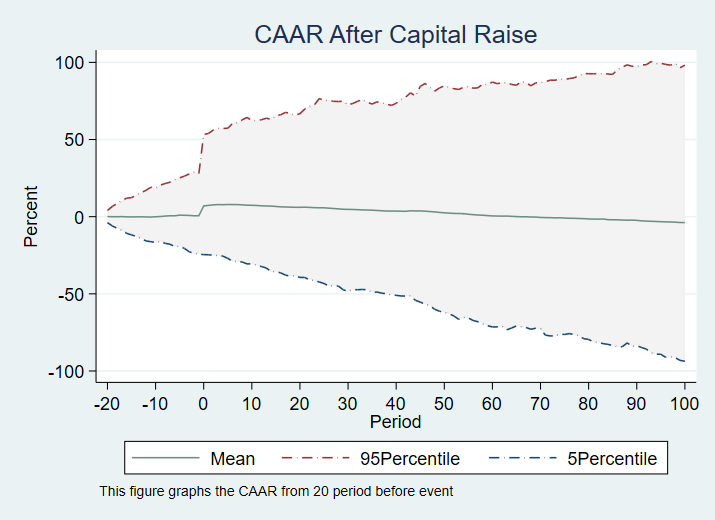
\includegraphics[width=0.7\linewidth]{95-5AbReturn.png}
	%\label{fig:95-5AbReturn}
	%\end{figure}
	%\end{frame}
	
	
	
	
	
	\begin{frame}{Abnormal Return}{Abnormal return of raised capital from Revaluation}
		\label{abreturnrevalution}
		\begin{figure}
			\centering
			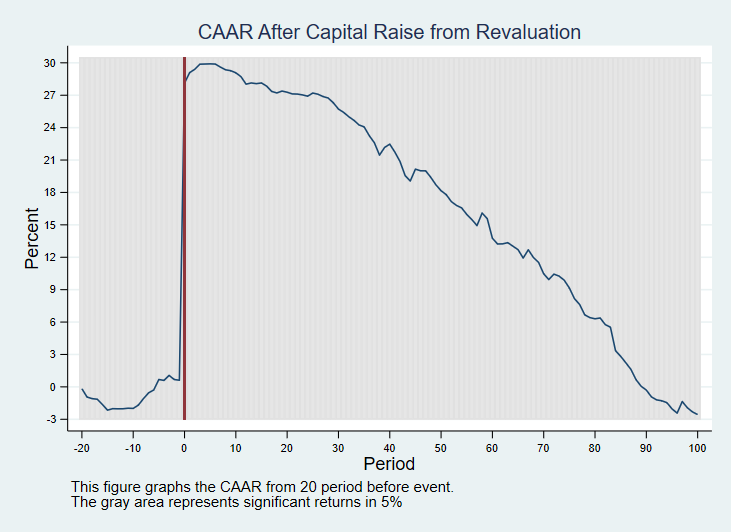
\includegraphics[width=0.65\linewidth]{Output/CARRevaluation.png}
			\label{fig:abreturnrevalution}
		\end{figure}

	\end{frame}
	
%	
%	\begin{frame}
%		
%		\centering
%		\begin{table}[htbp]
%			\centering
%			
%			\captionsetup{labelformat=empty}
%			\caption{\tiny Analysis of abnormal return in days surrounding the Revaluation announcements}
%			\resizebox{0.8\textheight}{!}
%			{\tiny
%				\begin{tabular}{cccc|cccc}
%					\hline\hline 
%					Period & \multicolumn{1}{c}{AAR} & \multicolumn{1}{c}{CAAR} & \multicolumn{1}{c}{t-stat} & Period & \multicolumn{1}{c}{AAR} & \multicolumn{1}{c}{CAAR} & \multicolumn{1}{c}{t-stat} \\
%					\hline
%					-20   & 0.04  & 0.04  & 0.13  & 0     & 28.55 & 29.18 & 6.41 \\
%					-19   & -0.89 & -0.86 & -2.02 & 1     & 1.08  & 30.26 & 6.58 \\
%					-18   & -0.26 & -1.08 & -1.83 & 2     & 0.35  & 30.61 & 6.58 \\
%					-17   & 0.11  & -0.97 & -1.50 & 3     & 0.47  & 31.08 & 6.55 \\
%					-16   & -0.39 & -1.36 & -1.82 & 4     & 0.17  & 31.25 & 6.43 \\
%					-15   & -0.52 & -1.88 & -2.26 & 5     & 0.10  & 31.36 & 6.34 \\
%					-14   & 0.21  & -1.67 & -1.72 & 6     & 0.07  & 31.42 & 6.26 \\
%					-13   & 0.00  & -1.67 & -1.48 & 7     & -0.40 & 31.02 & 6.11 \\
%					-12   & -0.14 & -1.81 & -1.40 & 8     & -0.28 & 30.74 & 6.01 \\
%					-11   & 0.02  & -1.80 & -1.35 & 9     & -0.07 & 30.67 & 5.90 \\
%					-10   & -0.15 & -1.95 & -1.45 & 10    & -0.02 & 30.65 & 5.83 \\
%					-9    & 0.33  & -1.61 & -1.15 & 11    & -0.38 & 30.27 & 5.66 \\
%					-8    & 0.72  & -0.89 & -0.59 & 12    & -0.59 & 29.68 & 5.59 \\
%					-7    & 0.67  & -0.22 & -0.14 & 13    & 0.21  & 29.89 & 5.62 \\
%					-6    & 0.33  & 0.12  & 0.07  & 14    & -0.15 & 29.49 & 5.39 \\
%					-5    & 0.63  & 0.75  & 0.44  & 15    & -0.02 & 29.47 & 5.34 \\
%					-4    & -0.16 & 0.58  & 0.32  & 16    & -0.43 & 29.05 & 5.21 \\
%					-3    & 0.30  & 0.89  & 0.43  & 17    & -0.61 & 28.43 & 5.09 \\
%					-2    & -0.26 & 0.63  & 0.29  & 18    & -0.17 & 28.27 & 5.02 \\
%					-1    & 0.01  & 0.63  & 0.28  & 19    & 0.39  & 28.65 & 5.03 \\
%					\hline\hline
%				\end{tabular}%
%			}
%		\end{table}%
%		
%		
%	\end{frame}
	
	
	
	\begin{frame}{Abnormal Return}{Abnormal return of raised capital from Reserves}
		\label{abreturnsaving}
		\begin{figure}
			\centering
			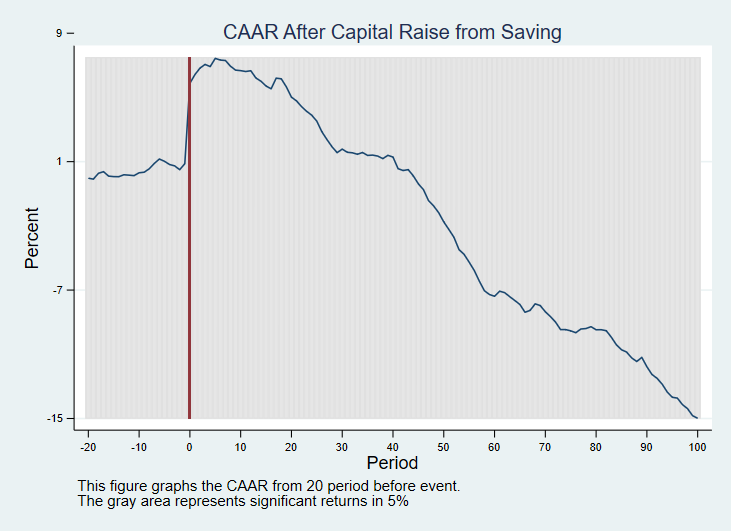
\includegraphics[width=0.65\linewidth]{Output/CARSaving.png}
			\label{fig:abreturnsaving}
		\end{figure}
		

	\end{frame}
	
	
	
	
	\begin{frame}{Abnormal Return}{Abnormal return of raised capital from Cash}
		\label{abreturncash}
		\begin{figure}
			\centering
			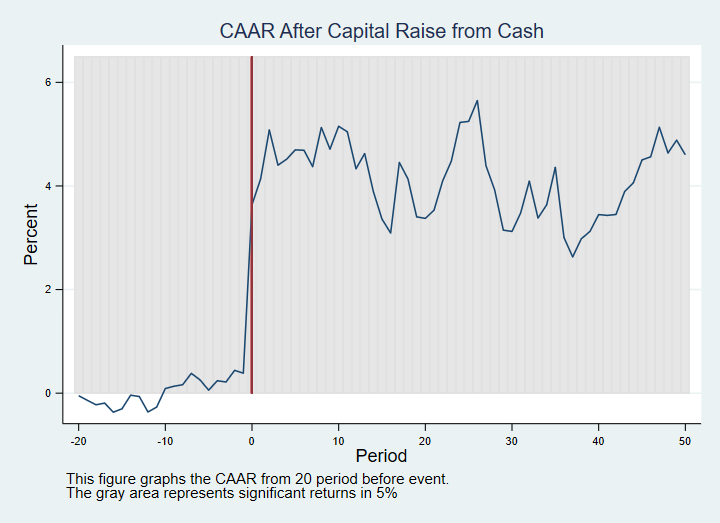
\includegraphics[width=0.65\linewidth]{Output/CARCash.png}
			\label{fig:abreturncash}
		\end{figure}

	\end{frame}
	
	
	
	
	
	\begin{frame}{Abnormal Return}{Abnormal return of raised capital from Cash \& Reserves}
		\label{abreturnhybrid}
		\begin{figure}
			\centering
			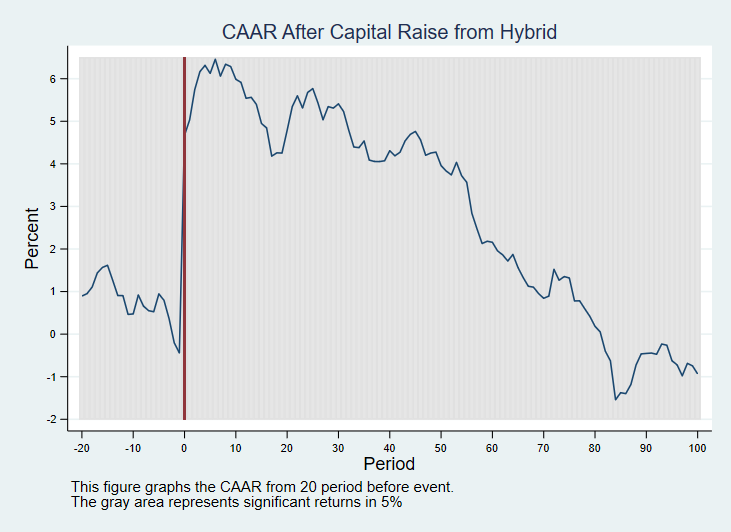
\includegraphics[width=0.65\linewidth]{Output/CARHybrid.png}
			\label{fig:abreturnhybrid}
		\end{figure}

	\end{frame}
	
	
	%\begin{frame}
	%\label{AbReturn_year}
	%\begin{figure}
	%\centering
	%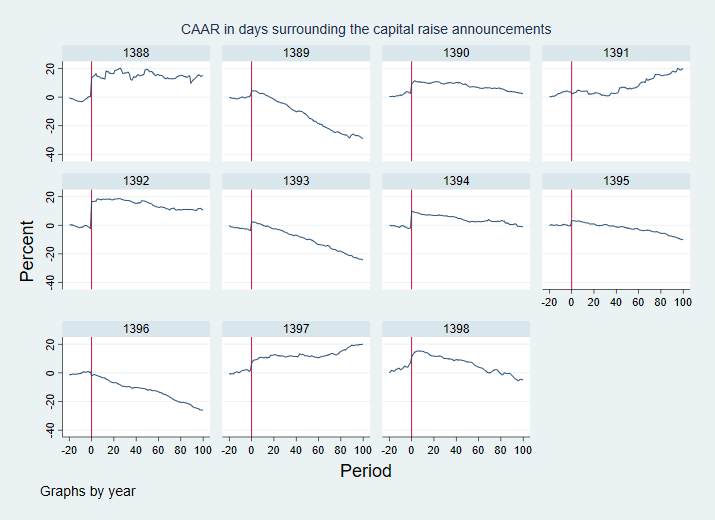
\includegraphics[width=0.85\linewidth]{AbReturn_year.png}
	%\label{fig:AbReturn_year}
	%\end{figure}
	%
	%
	%\end{frame}
	%
	%
	%\begin{frame}
	%\label{AbReturn_year_Revaluation}
	%\begin{figure}
	%\centering
	%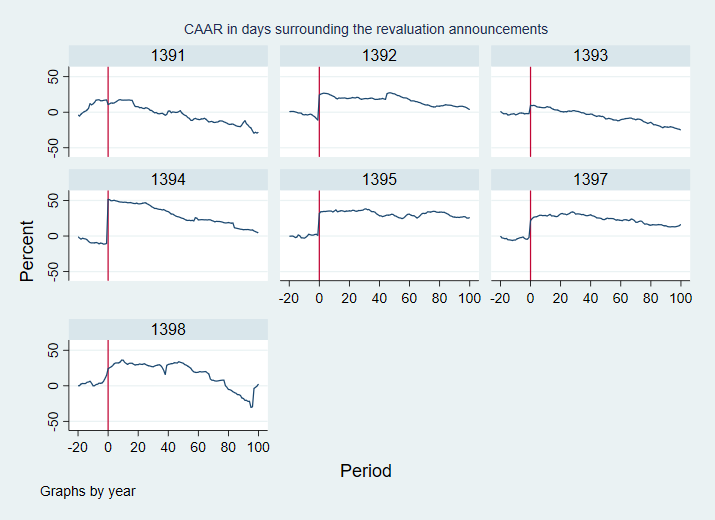
\includegraphics[width=0.85\linewidth]{AbReturn_year_Revaluation.png}
	%\label{fig:AbReturn_year_Revaluation}
	%\end{figure}
	%
	%
	%\end{frame}
	%
	%\begin{frame}
	%\label{AbReturn_year_NoRevaluation}
	%\begin{figure}
	%\centering
	%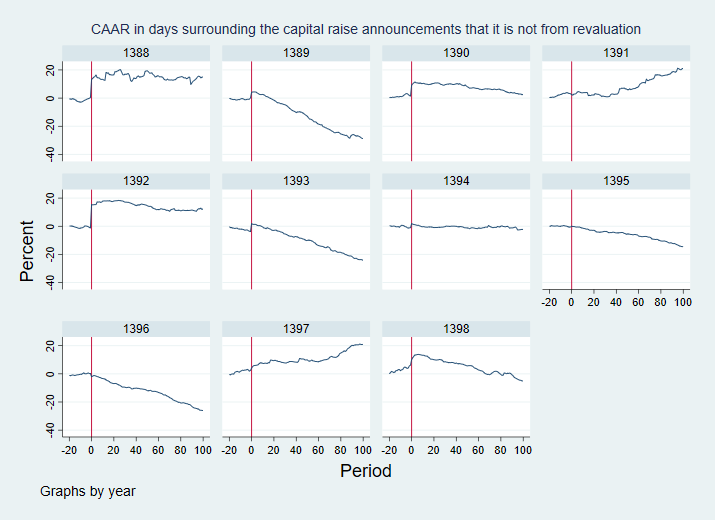
\includegraphics[width=0.85\linewidth]{AbReturn_year_NoRevaluation.png}
	%\label{fig:AbReturn_year_NoRevaluation}
	%\end{figure}
	%
	%
	%\end{frame}
	
	\subsection{Volume}
	
	\begin{frame}{Volume}
		\begin{figure}
			\centering
			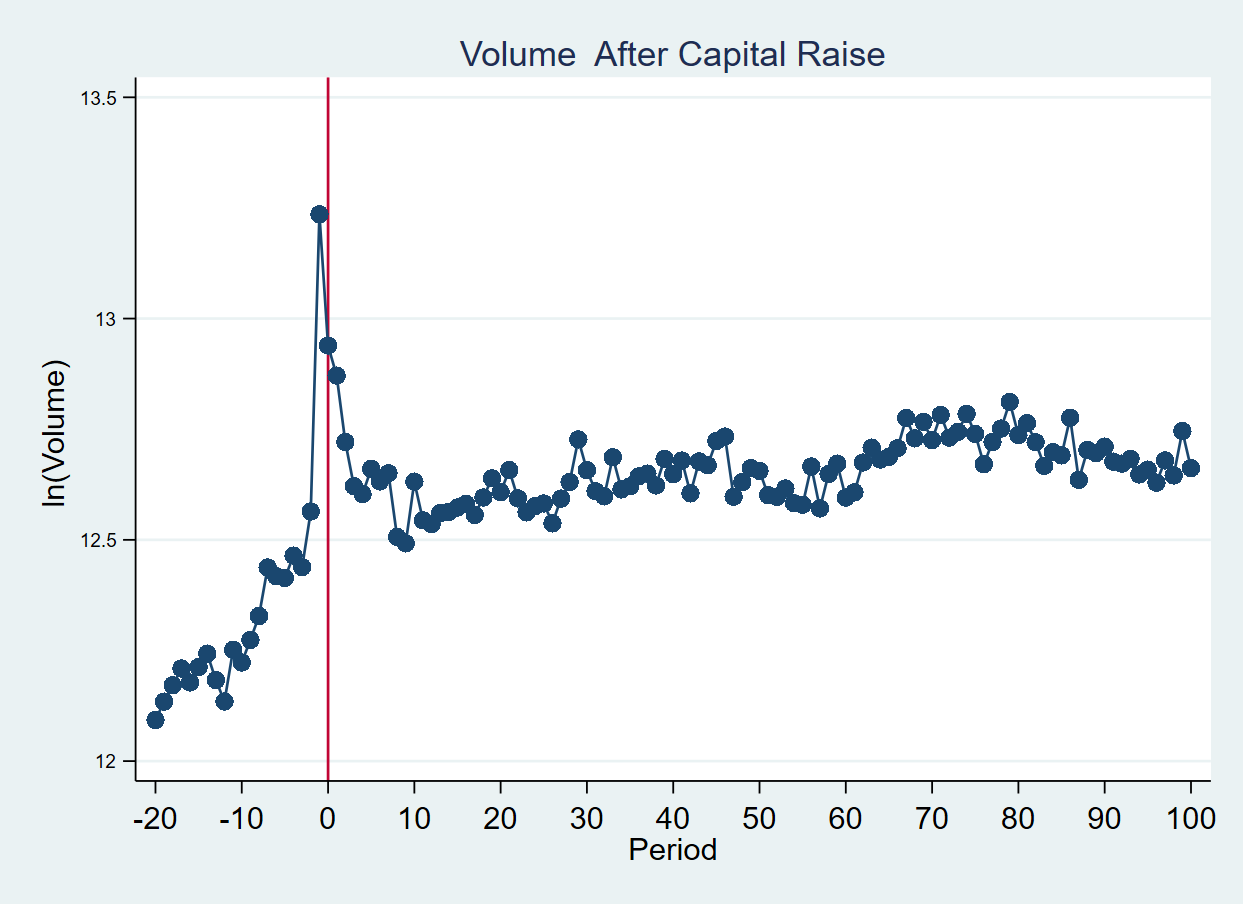
\includegraphics[width=0.7\linewidth]{Output/volume.png}
			\label{fig:volume}
		\end{figure}
	\end{frame}
	
	
	\begin{frame}{Volume}{Volume of raised capital from Revaluation}
		\begin{figure}
			\centering
			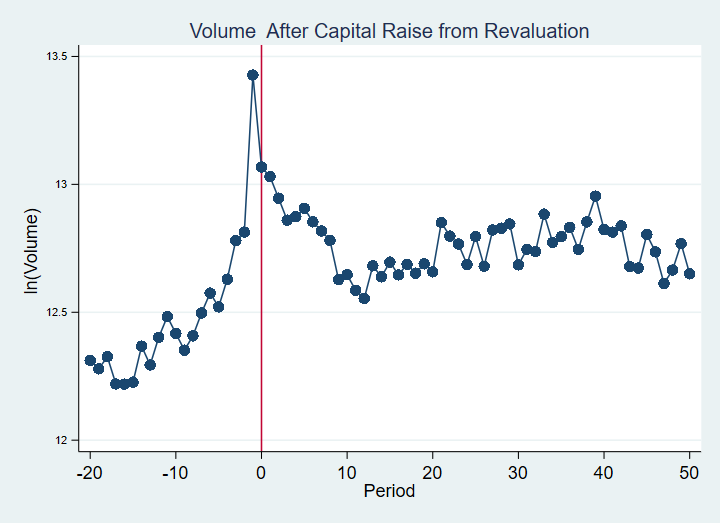
\includegraphics[width=0.7\linewidth]{Output/volume_Revaluation.png}
			\label{fig:volumerevaluation}
		\end{figure}
	\end{frame}
	
	
	\begin{frame}{Volume}{Volume of raised capital that it's not from Revaluation}
		\begin{figure}
			\centering
			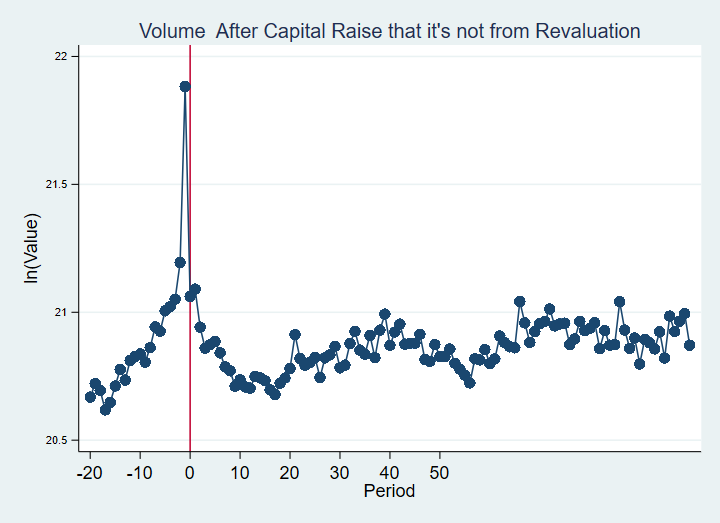
\includegraphics[width=0.7\linewidth]{Output/volume_NoRevaluation.png}
			\label{fig:volumenorevaluation}
		\end{figure}
	\end{frame}
	
	
	\subsection{Relative Volume}
	\begin{frame}{Relative volume}
		\begin{figure}
			\centering
			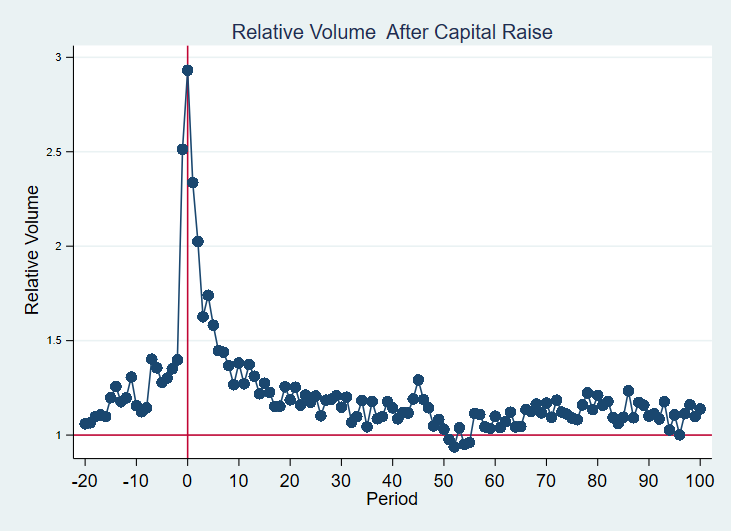
\includegraphics[width=0.7\linewidth]{Output/Relvolume.png}
			\label{fig:relvolume}
		\end{figure}
	\end{frame}
	\begin{frame}{Relative volume}{Relative Volume of raised capital from Revaluation}
		\begin{figure}
			\centering
			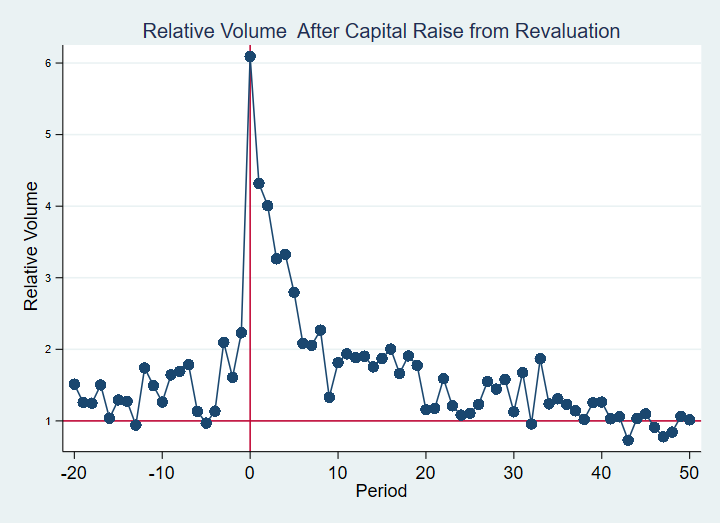
\includegraphics[width=0.7\linewidth]{Output/Relvolume_Revaluation.png}
			\label{fig:relvolumerevaluation}
		\end{figure}
	\end{frame}
	\begin{frame}{Relative volume}{Relative Volume of raised capital that it's not from Revaluation}
		\begin{figure}
			\centering
			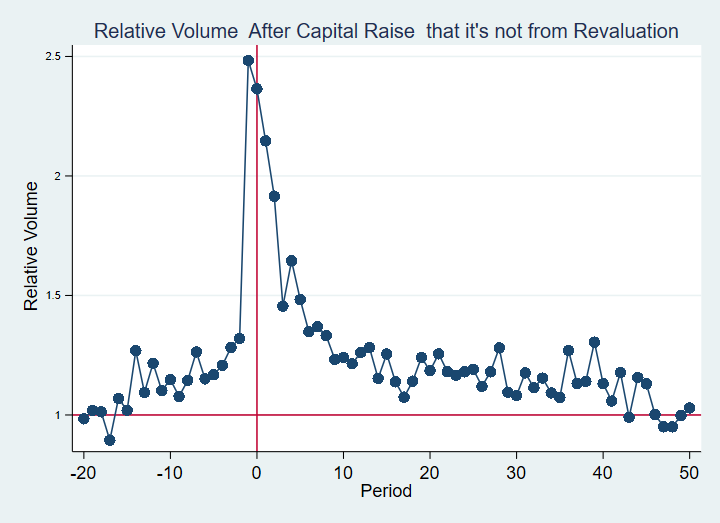
\includegraphics[width=0.7\linewidth]{Output/Relvolume_NoRevaluation.png}
			\label{fig:relvolumenorevaluation}
		\end{figure}
	\end{frame}
	
	
	
	\subsection{Buy-sell Imbalances}
	
	\begin{frame}{Buy-sell Imbalances}
		\begin{figure}
			\centering
			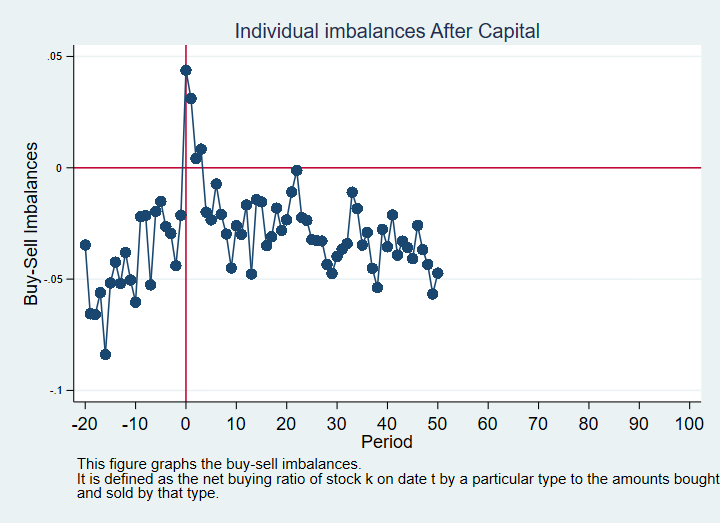
\includegraphics[width=0.45\linewidth]{Output/IndImb.png}
			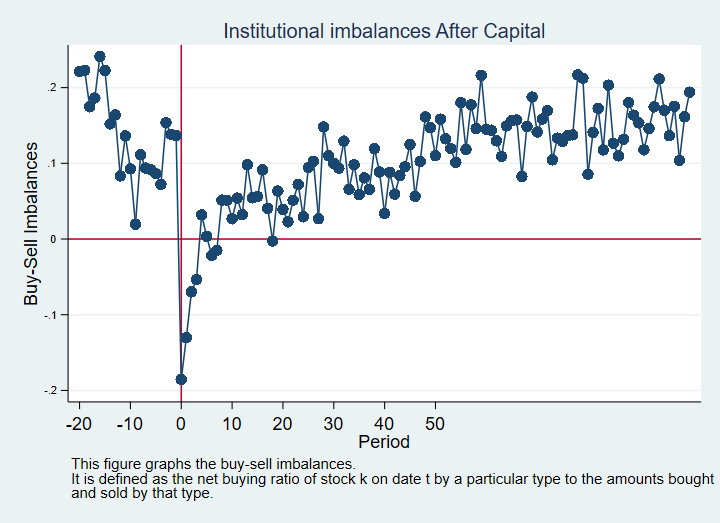
\includegraphics[width=0.45\linewidth]{Output/InsImb.png}
			\label{fig:indimb}
		\end{figure}
	\end{frame}
	\begin{frame}{Buy-sell Imbalances}{Buy-sell Imbalances of raised capital from Revaluation}
		\begin{figure}
			\centering
			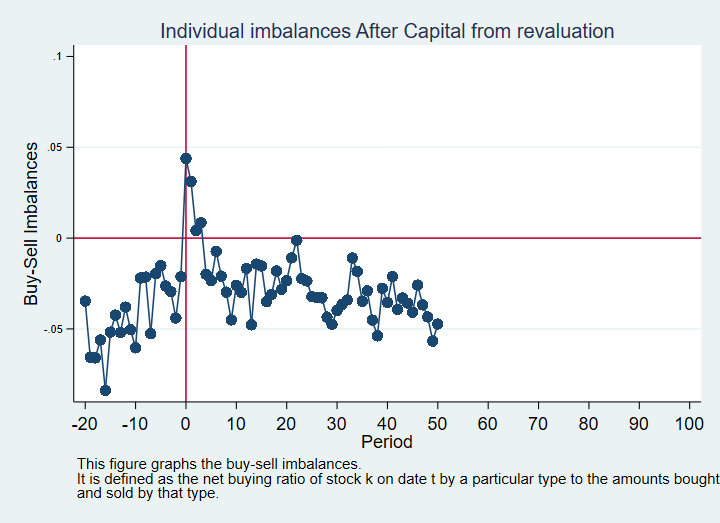
\includegraphics[width=0.45\linewidth]{Output/IndImb_Revaluation.png}
			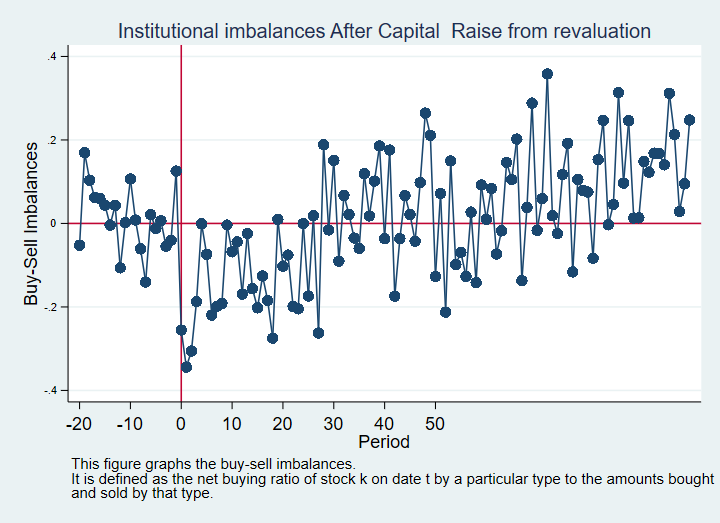
\includegraphics[width=0.45\linewidth]{Output/InsImb_Revaluation.png}
			\label{fig:indimbrevaluation}
		\end{figure}
	\end{frame}
	\begin{frame}{Buy-sell Imbalances}{Buy-sell Imbalances of raised capital that it's not from Revaluation}
		\begin{figure}
			\centering
			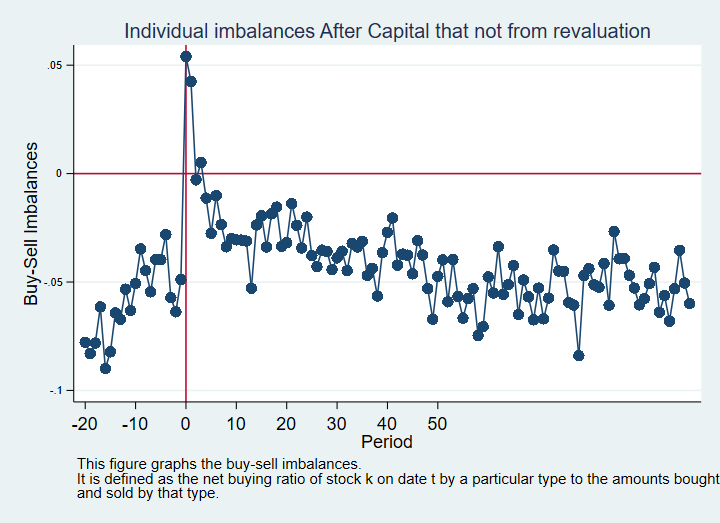
\includegraphics[width=0.45\linewidth]{Output/IndImb_NoRevaluation.png}
			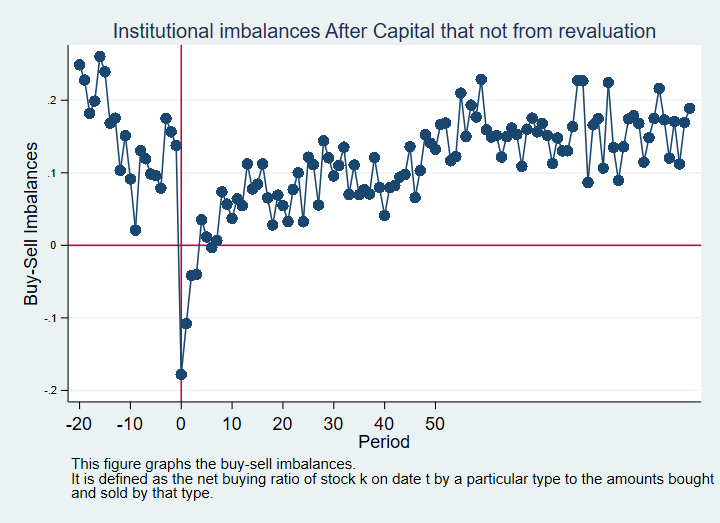
\includegraphics[width=0.45\linewidth]{Output/InsImb_NoRevaluation.png}
			\label{fig:indimbnorevaluation}
		\end{figure}
	\end{frame}
	
	\begin{frame}{Investors' Nav}{$ \text{Net buying volume}_{i,t} \times \text{ClosePrice}_{k,t} + \text{Net selling value}_{i,t} $}
		\begin{figure}
			\centering
			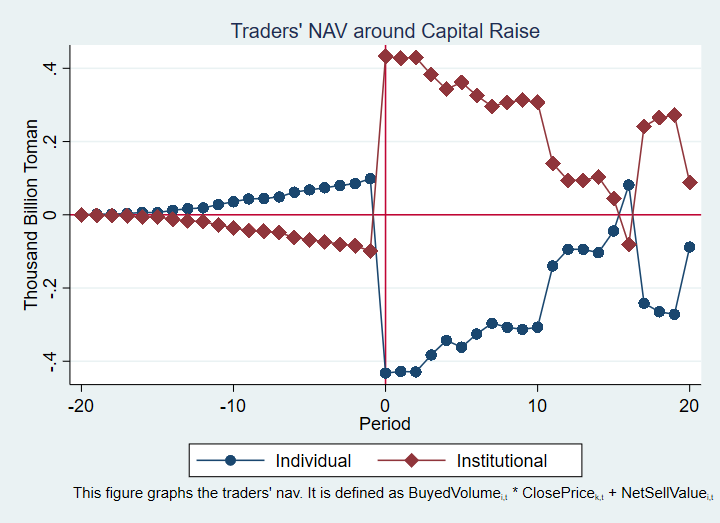
\includegraphics[width=0.65\linewidth]{Output/IndInsNav.png}
			\label{fig:IndInsNav}
		\end{figure}
	\end{frame}


	\begin{frame}{Investors' Nav}{$ \text{Net buying volume}_{i,t} \times \text{ClosePrice}_{k,t} + \text{Net selling value}_{i,t} $}
	\begin{figure}
		\centering
		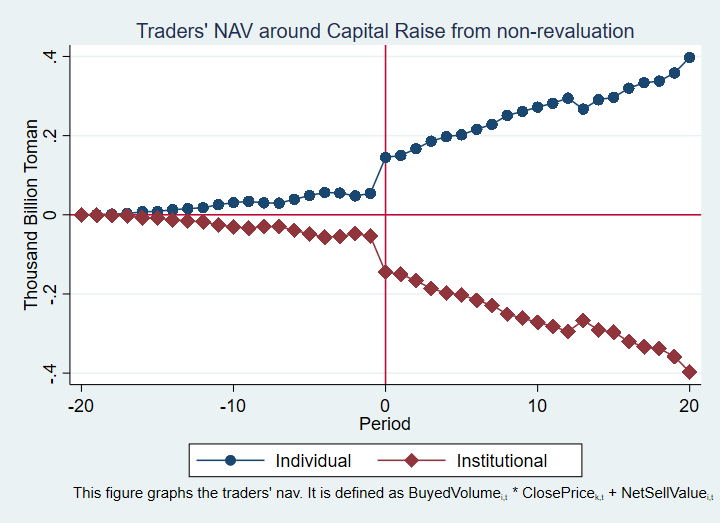
\includegraphics[width=0.45\linewidth]{Output/IndInsNav_NoRevaluation.png}
		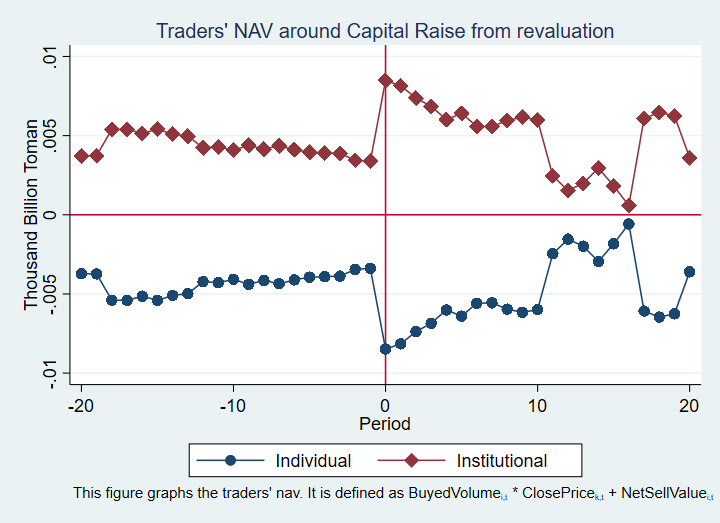
\includegraphics[width=0.45\linewidth]{Output/IndInsNav_Revaluation.png}
		\label{fig:IndInsNav_Revaluation}
	\end{figure}
\end{frame}
	
	
	
	\begin{frame}{Investors' Herding}{$LSV =  |br_{i,t} - \bar{br_{t}}| - E_t[|br_{i,t} - \bar{br_{t}}|] $}
		\begin{figure}
			\centering
			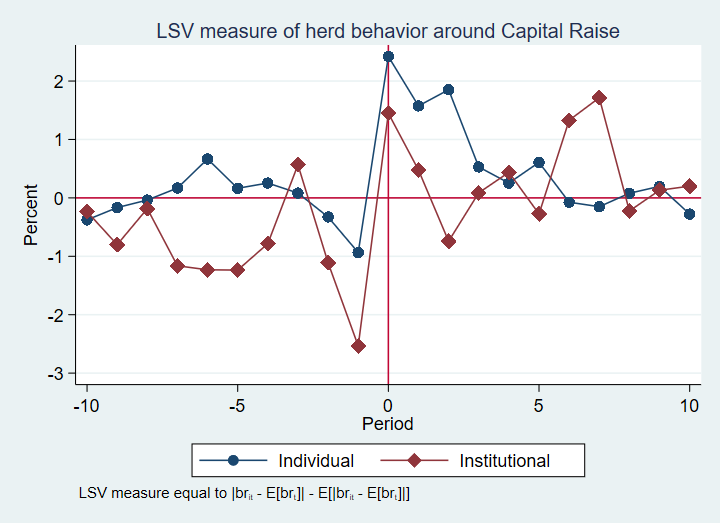
\includegraphics[width=0.65\linewidth]{Output/IndInsHerd.png}
			\label{fig:IndInsHerd}
		\end{figure}
	\end{frame}
	
		\begin{frame}{Investors' Herding}{$LSV =  |br_{i,t} - \bar{br_{t}}| - E_t[|br_{i,t} - \bar{br_{t}}|] $}
		\begin{figure}
			\centering
			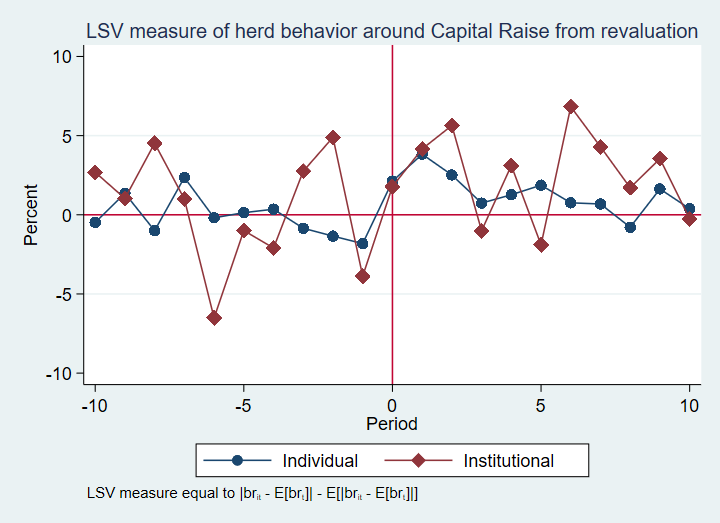
\includegraphics[width=0.45\linewidth]{Output/IndInsHerdRevaluation.png}
			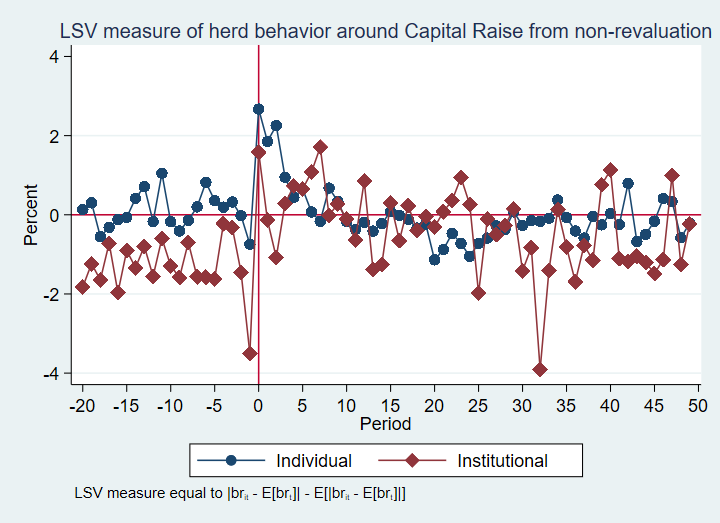
\includegraphics[width=0.45\linewidth]{Output/IndInsHerdNoRevaluation.png}
			\label{fig:IndInsHerd_Revaluation}
		\end{figure}
	\end{frame}
	
	
	
	\begin{frame}{Weight in Industry}
		\begin{figure}
			\centering
			\includegraphics[width=0.65\linewidth]{Output/weight}
			\label{fig:weight}
		\end{figure}
	\end{frame}
	
	
	
	
	\section{Cross Section}
	\begin{frame}
		\begin{columns}
			\column{0.48\textwidth}
			\begin{table}
				\centering
				\resizebox{1\textwidth}{!}{
					\begin{tabular}{lrrrrr}
\toprule
{} &   0-1 &   2-6 &  2-11 &  2-50 &  0-50 \\
IndNT\_Im &       &       &       &       &       \\
\midrule
1.0      &  4.20 &  0.35 &  0.00 & -2.82 &  1.37 \\
2.0      &  6.13 &  0.04 & -1.18 & -4.73 &  1.01 \\
3.0      &  3.52 &  0.62 &  0.30 & -4.22 & -0.19 \\
\bottomrule
\end{tabular}

				}
			
				\resizebox{1\textwidth}{!}{
				\begin{tabular}{lrrrrr}
\toprule
{} &   0-1 &   2-6 &  2-11 &  2-50 &  0-50 \\
IndNT\_Hm &       &       &       &       &       \\
\midrule
1.0      &  5.40 &  0.00 & -0.04 & -1.15 &  4.48 \\
2.0      &  3.84 &  0.69 & -0.09 & -3.56 &  0.49 \\
3.0      &  4.62 &  0.32 & -0.74 & -6.98 & -2.69 \\
\bottomrule
\end{tabular}

			}
			\end{table}
		\hfill
			\column{0.48\textwidth}
			\begin{table}
				\centering
				\resizebox{1\textwidth}{!}{
					\begin{tabular}{lrrrrr}
\toprule
{} &   0-1 &   2-6 &  2-11 &  2-50 &  0-50 \\
InsNT\_Im &       &       &       &       &       \\
\midrule
1.0      &  4.45 &  0.80 & -0.34 & -4.81 & -0.02 \\
2.0      &  6.36 &  0.27 & -0.04 & -4.64 &  1.39 \\
3.0      &  3.05 & -0.05 & -0.49 & -2.39 &  0.84 \\
\bottomrule
\end{tabular}

				}
			
			\resizebox{1\textwidth}{!}{
				\begin{tabular}{lrrrrr}
\toprule
{} &   0-1 &   2-6 &  2-11 &  2-50 &  0-50 \\
InsNT\_Hm &       &       &       &       &       \\
\midrule
1.0      &  2.16 & -0.17 & -0.59 & -4.09 & -1.75 \\
2.0      &  5.09 &  0.36 & -0.59 & -2.55 &  2.26 \\
3.0      &  6.60 &  0.83 &  0.31 & -5.01 &  1.78 \\
\bottomrule
\end{tabular}

			}
			\end{table}
		\end{columns}
	\end{frame}
\begin{frame}
\begin{columns}
	\column{0.5\textwidth}
	\begin{table}
		\centering
		\resizebox{1\textwidth}{!}{
			\begin{tabular}{lrrr}
\toprule
CAR(-10,-1) &   1.0 &   2.0 &   3.0 \\
InsNT\_Im &       &       &       \\
\midrule
1.0      & -5.37 & -0.71 &  4.02 \\
2.0      &  0.67 &  1.92 &  1.58 \\
3.0      & -3.86 &  3.48 &  2.86 \\
\bottomrule
\end{tabular}

		}
	\end{table}
	\column{0.5\textwidth}
	\begin{table}
		\centering
		\resizebox{1\textwidth}{!}{
			\begin{tabular}{lrrr}
\toprule
CAR(-10,-1) &   1.0 &   2.0 &   3.0 \\
IndNT\_Im &       &       &       \\
\midrule
1.0      & -2.51 &  2.05 &  4.57 \\
2.0      & -0.58 &  2.07 &  1.89 \\
3.0      & -6.09 &  1.25 &  2.54 \\
\bottomrule
\end{tabular}

		}
	\end{table}
\end{columns}			
\end{frame}
	
\begin{frame}
	\begin{columns}
		\column{0.5\textwidth}
		\begin{table}
			\centering
			\resizebox{1\textwidth}{!}{
				\begin{tabular}{lrrrrr}
\toprule
{} &   0-1 &   2-6 &  2-11 &  2-50 &  0-50 \\
Grouped &       &       &       &       &       \\
\midrule
0       &  4.97 &  0.41 & -0.08 & -4.41 &  0.81 \\
1       &  3.88 &  0.20 & -0.73 & -2.89 &  0.57 \\
\bottomrule
\end{tabular}

			}
		\end{table}
		\column{0.5\textwidth}
		\begin{table}
			\centering
			\resizebox{1\textwidth}{!}{
				\begin{tabular}{lrrrrr}
\toprule
{} &   0-1 &   2-6 &  2-11 &  2-50 &  0-50 \\
Excess &       &       &       &       &       \\
\midrule
2.0    &  3.80 &  1.37 &  0.83 & -2.25 &  1.61 \\
3.0    &  4.05 & -2.14 & -3.86 & -4.36 & -1.81 \\
\bottomrule
\end{tabular}

			}
		\end{table}
	\end{columns}			
\end{frame}	
	
	
	
	
	
	
	
	
	
	
	
	
	
	%\section{Abnormal Return Analysis}
	%\def\sym#1{\ifmmode^{#1}\else\(^{#1}\)\fi}
	%\begin{frame}
	%\begin{center}
	%
	%\begin{columns}
	%
	%\column{.5\textwidth}     
	% \centering
	% \resizebox{0.7\textwidth}{!}{
	%         \begin{tabular}{CCCC}
	%         \toprule\toprule
	%         \multicolumn{4}{c}{\textit{Abnormal Return at event day }} \\
	%                \multicolumn{4}{c}{\scriptsize\textit{Panel A:}{ Market Cap}}\\
	%                \hline\hline
	%               & \multicolumn{2}{c}{\scriptsize Revaluation}        &  \\
	%               \cmidrule{2-3}
	%         \multicolumn{1}{l}{Sub sample} & \multicolumn{1}{c}{No} & \multicolumn{1}{c}{Yes} & \multicolumn{1}{c}{Total} \\
	%          \hline
	%    \rowfont{\normalsize}%
	%    Small & 6.73  & 39.64 & 9.48 \\
	%    \rowfont{\scriptsize}%
	%      sd    & 19.66 & 40.16 & 23.82 \\
	%        n  & 285   & 26    & 311 \\
	%          \hline
	%    \rowfont{\normalsize}%      
	%    Middle & 3.73  & 37.33 & 6.47 \\
	%    \rowfont{\scriptsize}%
	%       sd   & 12.88 & 41.20 & 19.24 \\
	%       n  & 282   & 25    & 307 \\
	%          \hline
	%          \rowfont{\normalsize}%
	%    Large & 2.37  & 12.68 & 3.38 \\
	%    \rowfont{\scriptsize}%
	%       sd   & 11.21 & 16.96 & 12.26 \\
	%       n   & 293   & 32    & 325 \\
	%          \hline
	%          \rowfont{\normalsize}%
	%    Full sample & 4.26  & 28.55 & 6.40 \\
	%    \rowfont{\scriptsize}%
	%      sd    & 15.11 & 35.47 & 19.10 \\
	%       n   & 860   & 83    & 943 \\
	%          \hline
	%          \rowfont{\normalsize}%
	%    Small - Large & 4.366\sym{***} & 26.96\sym{**} & 6.101\sym{***} \\
	%   \scriptsize P-Value & 0.001 & 0.003 & 0 \\
	%     \bottomrule\bottomrule
	%     \addlinespace[.75ex]
	%     \end{tabular}
	% }
	% 
	% \column{.5\textwidth}     
	%  \centering
	%   \resizebox{0.58\textwidth}{!}{
	%      \begin{tabular}{CCCC}
	%               \toprule\toprule
	%               \multicolumn{4}{c}{\textit{Abnormal Return at event day }} \\
	%                      \multicolumn{4}{c}{\scriptsize\textit{Panel B:} {P/E ratio}}\\
	%                      \hline\hline
	%                     & \multicolumn{2}{c}{\scriptsize Revaluation}        &  \\
	%                     \cmidrule{2-3}
	%               \multicolumn{1}{l}{Sub sample} & \multicolumn{1}{c}{No} & \multicolumn{1}{c}{Yes} & \multicolumn{1}{c}{Total} \\
	%                \hline
	%                \rowfont{\normalsize}%
	%   {Low} & 2.39  & 35.88 & 4.99 \\
	%   \rowfont{\scriptsize}%
	%       sd   & 15.22 & 42.50 & 20.67 \\
	%        n  & 214   & 18    & 232 \\\hline\rowfont{\normalsize}%
	%    {Middle} & 4.76  & 37.58 & 7.07 \\
	%       sd   & 20.26 & 41.74 & 23.84 \\
	%        n  & 224   & 17    & 241 \\\hline\rowfont{\normalsize}%
	%    {High} & 3.83  & 18.20 & 5.14 \\\rowfont{\scriptsize}%
	%       sd   & 9.95  & 23.17 & 12.41 \\
	%       n   & 219   & 22    & 241 \\\hline\rowfont{\normalsize}%
	%    {Full sample} & 3.68  & 29.56 & 5.74 \\\rowfont{\scriptsize}%
	%       sd   & 15.77 & 36.48 & 19.56 \\
	%       n   & 657   & 57    & 714 \\ 
	%          \hline \rowfont{\normalsize}%
	%    {Low - High} & -1.436 & 17.68 & -0.149 \\\rowfont{\scriptsize}%
	%    {P-Value}     & 0.247 & 0.126 & 0.924 \\           
	%           \bottomrule\bottomrule
	%           \addlinespace[.75ex]
	%           \end{tabular}
	%       }
	%
	%
	% 
	%\end{columns}
	%
	%\normalsize
	%\end{center}
	%\end{frame}
	%
	%
	%\begin{frame}
	%\begin{center}
	%
	%\begin{columns}
	%\column{.5\textwidth}     
	% \centering
	% 
	%  \resizebox{0.6\textwidth}{!}{
	%          \begin{tabular}{CCCC}
	%          \toprule\toprule
	%          \multicolumn{4}{c}{\textit{Abnormal Return at event day }} \\
	%                 \multicolumn{4}{c}{\scriptsize\textit{Panel C:}{ Book-to-Market}}\\
	%                 \hline\hline
	%                & \multicolumn{2}{c}{\scriptsize Revaluation}        &  \\
	%                \cmidrule{2-3}
	%          \multicolumn{1}{l}{Sub sample} & \multicolumn{1}{c}{No} & \multicolumn{1}{c}{Yes} & \multicolumn{1}{c}{Total} \\
	%           \hline\rowfont{\normalsize}%
	%          {Low} & 5.48  & 36.85 & 8.08 \\\rowfont{\scriptsize}%
	%            sd    & 19.07 & 47.28 & 24.23 \\
	%             n   & 288   & 26    & 314 \\
	%                 \hline\rowfont{\normalsize}%
	%          {Middle} & 3.14  & 28.41 & 5.03 \\\rowfont{\scriptsize}%
	%             sd   & 12.87 & 33.15 & 16.62 \\
	%             n   & 285   & 23    & 308 \\
	%                 \hline\rowfont{\normalsize}%
	%          {High} & 4.15  & 22.30 & 6.07 \\\rowfont{\scriptsize}%
	%             sd   & 12.38 & 24.60 & 15.18 \\
	%             n   & 287   & 34    & 321 \\
	%                 \hline\rowfont{\normalsize}%
	%          {Full sample} & 4.26  & 28.55 & 6.40 \\\rowfont{\scriptsize}%
	%             sd   & 15.11 & 35.47 & 19.10 \\
	%              n  & 860   & 83    & 943 \\
	%                \hline\rowfont{\normalsize}%
	%         {Low - High} & 1.327 & 14.55 & 2.003 \\\rowfont{\scriptsize}%
	%          {P-Value}      & 0.323 & 0.162 & 0.214 \\
	%      \bottomrule\bottomrule
	%      \addlinespace[.75ex]
	%      \end{tabular}
	%  }
	%  
	%  
	% 
	% \column{.5\textwidth}     
	%  \centering
	%   \resizebox{0.6\textwidth}{!}{
	%      \begin{tabular}{CCCC}
	%               \toprule\toprule
	%               \multicolumn{4}{c}{\textit{Abnormal Return at event day }} \\
	%                      \multicolumn{4}{c}{\scriptsize\textit{Panel D:}{ Free Float}}\\
	%                      \hline\hline
	%                     & \multicolumn{2}{c}{\scriptsize Revaluation}        &  \\
	%                     \cmidrule{2-3}
	%               \multicolumn{1}{l}{Sub sample} & \multicolumn{1}{c}{No} & \multicolumn{1}{c}{Yes} & \multicolumn{1}{c}{Total} \\
	%                \hline\rowfont{\normalsize}%
	%    Low   & 5.13  & 21.17 & 6.59 \\\rowfont{\scriptsize}%
	%      sd    & 19.60 & 23.58 & 20.48 \\
	%        n  & 271   & 27    & 298 \\\hline\rowfont{\normalsize}%
	%    Middle & 3.39  & 28.43 & 5.31 \\\rowfont{\scriptsize}%
	%       sd   & 12.62 & 41.21 & 17.79 \\
	%       n   & 277   & 23    & 300 \\\hline\rowfont{\normalsize}%
	%    High  & 4.20  & 35.52 & 7.32 \\\rowfont{\scriptsize}%
	%       sd   & 12.45 & 39.95 & 19.54 \\
	%        n  & 281   & 31    & 312 \\\hline\rowfont{\normalsize}%
	%    Full sample & 4.24  & 28.72 & 6.42 \\
	%        sd  & 15.21 & 35.83 & 19.30 \\\rowfont{\scriptsize}%
	%        n  & 829   & 81    & 910 \\
	%          \hline\rowfont{\normalsize}%
	%    Low - High &  0.929 & -14.35 & -0.73 \\\rowfont{\scriptsize}%
	%    P-Value &0.508  &  0.097 & 0.653 \\        
	%           \bottomrule\bottomrule
	%           \addlinespace[.75ex]
	%           \end{tabular}
	%       }
	%\end{columns}
	%
	%\normalsize
	%\end{center}
	%\end{frame}
	%
	%
	%
	%
	%\begin{frame}
	%\begin{center}
	%
	%\begin{columns}
	%\column{.5\textwidth}     
	% \centering
	% \resizebox{0.75\textwidth}{!}{
	%         \begin{tabular}{CCCC}
	%         \toprule\toprule
	%         \multicolumn{4}{c}{\textit{Abnormal Return at event day }} \\
	%                \multicolumn{4}{c}{\scriptsize\textit{Panel E: }{ Free Market Cap}}\\
	%                \hline\hline
	%               & \multicolumn{2}{c}{\scriptsize Revaluation}        &  \\
	%               \cmidrule{2-3}
	%         \multicolumn{1}{l}{Sub sample} & \multicolumn{1}{c}{No} & \multicolumn{1}{c}{Yes} & \multicolumn{1}{c}{Total} \\
	%          \hline\rowfont{\normalsize}
	%    Small & 6.11  & 40.98 & 9.36 \\\rowfont{\scriptsize}
	%       sd   & 20.10 & 46.67 & 25.81 \\
	%       n   & 272   & 28    & 300 \\ \hline\rowfont{\normalsize}
	%    Middle & 4.39  & 27.42 & 6.11 \\\rowfont{\scriptsize}
	%       sd   & 13.36 & 30.56 & 16.39 \\
	%        n  & 273   & 22    & 295 \\ \hline\rowfont{\normalsize}
	%    Large & 2.30  & 18.58 & 3.90 \\\rowfont{\scriptsize}
	%       sd   & 10.54 & 23.67 & 13.31 \\
	%       n   & 284   & 31    & 315 \\ \hline\rowfont{\normalsize}
	%    Full sample & 4.24  & 28.72 & 6.42 \\\rowfont{\scriptsize}
	%       sd   & 15.21 & 35.83 & 19.30 \\
	%       n   & 829   & 81    & 910 \\ \hline\rowfont{\normalsize}
	%    Small - Large & 3.813\sym{**} & 22.41\sym{***} & 5.466\sym{***} \\\rowfont{\scriptsize}
	%    P-Value & 0.006 & 0.028 & 0.001 \\
	%     \bottomrule\bottomrule
	%     \addlinespace[.75ex]
	%     \end{tabular}
	% }
	% 
	% 
	% \column{.5\textwidth}     
	%  \centering
	%   \resizebox{0.6\textwidth}{!}{
	%      \begin{tabular}{CCCC}
	%               \toprule\toprule
	%               \multicolumn{4}{c}{\textit{Abnormal Return at event day }} \\
	%                      \multicolumn{4}{c}{\scriptsize\textit{Panel F:}{ Volatility(past 250 days)}}\\
	%                      \hline\hline
	%                     & \multicolumn{2}{c}{\scriptsize Revaluation}        &  \\
	%                     \cmidrule{2-3}
	%               \multicolumn{1}{l}{Sub sample} & \multicolumn{1}{c}{No} & \multicolumn{1}{c}{Yes} & \multicolumn{1}{c}{Total} \\
	%                \hline\rowfont{\normalsize}
	%    Low   & 4.50  & 24.11 & 6.29 \\\rowfont{\scriptsize}
	%      sd    & 18.72 & 28.69 & 20.56 \\
	%       n   & 269   & 27    & 296 \\\hline\rowfont{\normalsize}
	%    Middle & 4.90  & 34.68 & 7.32 \\\rowfont{\scriptsize}
	%        sd  & 12.28 & 33.07 & 17.04 \\
	%       n   & 260   & 23    & 283 \\\hline\rowfont{\normalsize}
	%    High  & 2.68  & 23.08 & 4.82 \\\rowfont{\scriptsize}
	%       sd   & 13.92 & 34.70 & 18.31 \\
	%       n   & 264   & 31    & 295 \\\hline\rowfont{\normalsize}
	%    Full sample & 4.02  & 26.72 & 6.13 \\\rowfont{\scriptsize}
	%      sd    & 15.27 & 32.33 & 18.73 \\
	%       n   & 793   & 81    & 874 \\\hline\rowfont{\normalsize}
	%    Low - High & 1.823 & 1.037 & 1.468 \\\rowfont{\scriptsize}
	%    P-Value & 0.202 & 0.901 & 0.36 \\      
	%           \bottomrule\bottomrule
	%           \addlinespace[.75ex]
	%           \end{tabular}
	%       }
	%\end{columns}
	%
	%
	%\normalsize
	%\end{center}
	%\end{frame}
	%
	%
	%
	%\begin{frame}
	%\begin{center}
	%
	%\begin{columns}
	%\column{.5\textwidth}     
	% \centering
	% \resizebox{0.6\textwidth}{!}{
	%         \begin{tabular}{CCCC}
	%         \toprule\toprule
	%         \multicolumn{4}{c}{\textit{Abnormal Return at event day }} \\
	%                \multicolumn{4}{c}{\scriptsize\textit{Panel G: }{Debt ratio}}\\
	%                \hline\hline
	%               & \multicolumn{2}{c}{\scriptsize Revaluation}        &  \\
	%               \cmidrule{2-3}
	%         \multicolumn{1}{l}{Sub sample} & \multicolumn{1}{c}{No} & \multicolumn{1}{c}{Yes} & \multicolumn{1}{c}{Total} \\
	%          \hline\rowfont{\normalsize}
	%    Low   & 4.19  & 34.87 & 6.80 \\\rowfont{\scriptsize}
	%      sd    & 18.95 & 43.56 & 23.61 \\
	%       n   & 280   & 26    & 306 \\\hline\rowfont{\normalsize}
	%    Middle & 3.69  & 28.19 & 5.67 \\\rowfont{\scriptsize}
	%       sd   & 11.93 & 25.80 & 15.07 \\
	%       n   & 273   & 24    & 297 \\\hline\rowfont{\normalsize}
	%    High  & 5.06  & 23.42 & 6.80 \\\rowfont{\scriptsize}
	%       sd   & 14.24 & 36.81 & 18.36 \\
	%        n  & 277   & 29    & 306 \\\hline\rowfont{\normalsize}
	%    Full sample & 4.32  & 28.64 & 6.43 \\\rowfont{\scriptsize}
	%       sd   & 15.34 & 36.25 & 19.36 \\
	%       n   & 830   & 79    & 909 \\\hline\rowfont{\normalsize}
	%    Low - High & -0.872 & 11.45 & -0.005 \\\rowfont{\scriptsize}
	%    P-Value & 0.539 & 0.301 & 0.998 \\
	%     \bottomrule\bottomrule
	%     \addlinespace[.75ex]
	%     \end{tabular}
	% }
	% 
	% 
	% \column{.5\textwidth}     
	%  \centering
	%   \resizebox{0.6\textwidth}{!}{
	%      \begin{tabular}{CCCC}
	%               \toprule\toprule
	%               \multicolumn{4}{c}{\textit{Abnormal Return at event day }} \\
	%                      \multicolumn{4}{c}{\scriptsize\textit{Panel H:}{ Leverage ratio}}\\
	%                      \hline\hline
	%                     & \multicolumn{2}{c}{\scriptsize Revaluation}        &  \\
	%                     \cmidrule{2-3}
	%               \multicolumn{1}{l}{Sub sample} & \multicolumn{1}{c}{No} & \multicolumn{1}{c}{Yes} & \multicolumn{1}{c}{Total} \\
	%                \hline\rowfont{\normalsize}
	%    Low   & 3.80  & 29.24 & 5.97 \\\rowfont{\scriptsize}
	%      sd    & 10.37 & 31.09 & 15.13 \\
	%       n   & 278   & 26    & 304 \\\hline\rowfont{\normalsize}
	%    Middle & 3.84  & 23.49 & 5.36 \\\rowfont{\scriptsize}
	%       sd   & 12.64 & 29.34 & 15.46 \\
	%       n   & 274   & 23    & 297 \\\hline\rowfont{\normalsize}
	%    High  & 5.31  & 32.06 & 7.92 \\\rowfont{\scriptsize}
	%      sd    & 20.93 & 44.88 & 25.47 \\
	%      b    & 278   & 30    & 308 \\\hline\rowfont{\normalsize}
	%    Full sample & 4.32  & 28.64 & 6.43 \\\rowfont{\scriptsize}
	%       sd   & 15.34 & 36.25 & 19.36 \\
	%       n   & 830   & 79    & 909 \\\hline\rowfont{\normalsize}
	%    Low - High & -1.512 & -2.817 & -1.941 \\\rowfont{\scriptsize}
	%    P-Value & 0.281 & 0.784 & 0.251 \\      
	%           \bottomrule\bottomrule
	%           \addlinespace[.75ex]
	%           \end{tabular}
	%       }
	%\end{columns}
	%
	%
	%\normalsize
	%\end{center}
	%\end{frame}
	%
	%
	%\begin{frame}
	%\begin{center}
	%
	% \resizebox{0.25\textwidth}{!}{
	%         \begin{tabular}{CCCC}
	%         \toprule\toprule
	%         \multicolumn{4}{c}{\textit{Abnormal Return at event day }} \\
	%                \multicolumn{4}{c}{\scriptsize\textit{Panel I: }{Market Condition}}\\
	%                \hline\hline
	%               & \multicolumn{2}{c}{\scriptsize Revaluation}        &  \\
	%               \cmidrule{2-3}
	%         \multicolumn{1}{l}{Sub sample} & \multicolumn{1}{c}{No} & \multicolumn{1}{c}{Yes} & \multicolumn{1}{c}{Total} \\
	%          \hline\rowfont{\normalsize}
	%    {Bad} & 3.85  & 29.85 & 6.20 \\\rowfont{\scriptsize}
	%      sd    & 12.96 & 37.65 & 18.25 \\
	%        n  & 301   & 30    & 331 \\\hline\rowfont{\normalsize}
	%    {Good} & 4.48  & 27.82 & 6.51 \\\rowfont{\scriptsize}
	%       sd   & 16.15 & 34.52 & 19.56 \\
	%        n  & 559   & 53    & 612 \\\hline\rowfont{\normalsize}
	%    {Full sample} & 4.26  & 28.55 & 6.40 \\\rowfont{\scriptsize}
	%        sd  & 15.11 & 35.47 & 19.10 \\
	%        n  & 860   & 83    & 943 \\
	%     \bottomrule\bottomrule
	%     \addlinespace[.75ex]
	%     \end{tabular}
	% }
	%
	%
	%\normalsize
	%\end{center}
	%\end{frame}
	
	
	%\begin{frame}
	%\begin{center}
	%\footnotesize
	%\newcolumntype{Y}{>{\raggedleft\arraybackslash}X}
	%\resizebox{0.8\textwidth}{!}{
	%\begin{tabularx} {15cm} {@{}  l Y Y Y Y Y Y@{}} 
	%\toprule\toprule
	%\multicolumn{7}{c}{\textit{Mean of Abnormal Return}} \\
	%\hline\hline
	% & \multicolumn{6}{c}{\scriptsize P/E Quantile} \\
	%\cmidrule{2-6} \scriptsize Size Quantile&$ 1_\text{\tiny (Low)} $&2&3&4&$ 5_\text{\tiny (High)} $&Row average \\
	%\hline
	%$ 1_\text{\tiny (Low)} $&17.0&11.8&29.9&8.5&7.9&13.3 \\
	%2&15.0&8.1&3.0&8.7&5.4&8.0 \\
	%3&0.3&-0.5&5.3&6.5&6.8&4.0 \\
	%4&-2.3&2.2&-1.1&3.0&3.1&0.9 \\
	%$ 5_\text{\tiny (High)} $&2.4&-0.4&3.6&1.1&7.5&2.6 \\
	%Column average&7.1&3.3&5.1&5.7&6.0&5.4 \\
	%
	%\bottomrule\bottomrule
	%\addlinespace[.75ex]
	%\end{tabularx}
	%}
	%\par
	%
	%\normalsize
	%\end{center}
	%\end{frame}
	%
	%\begin{frame}
	%
	%\begin{center}
	%\footnotesize
	%\newcolumntype{Y}{>{\raggedleft\arraybackslash}X}
	%\resizebox{0.8 \textwidth}{!}{
	%\begin{tabularx} {15cm} {@{} l Y Y Y Y Y Y@{}} 
	%\toprule \toprule
	%\multicolumn{7}{c}{\textit{Mean of Abnormal Return}} \\
	%\hline\hline
	% & \multicolumn{6}{c}{\scriptsize Book-to-Market Quantile} \\
	%\cmidrule{2-6} \scriptsize P/E Quantile &$ 1_\text{\tiny (Low)} $&2&3&4&$ 5_\text{\tiny (High)} $&Row average \\
	%\hline
	%$ 1_\text{\tiny (Low)} $&15.4&3.3&3.7&6.3&4.6&7.1 \\
	%2&4.0&2.9&5.1&2.0&1.6&3.3 \\
	%3&11.8&4.3&1.5&2.5&4.2&5.1 \\
	%4&4.8&6.5&2.8&8.6&5.5&5.7 \\
	%$ 5_\text{\tiny (High)} $&10.2&7.0&2.9&4.8&5.9&6.0 \\
	%Column average&9.6&4.7&3.3&4.6&4.8&5.4 \\
	%\bottomrule
	%\bottomrule
	%\addlinespace[.75ex]
	%\end{tabularx}
	%}
	%\par
	%\normalsize
	%\end{center}
	%
	%\end{frame}
	
	
	
	
	
	%\begin{frame}
	%\begin{table}[htbp]
	%\centering
	%    \resizebox{0.4\textheight}{!}{
	%{
\def\sym#1{\ifmmode^{#1}\else\(^{#1}\)\fi}
\begin{tabular}{l*{4}{c}}
\hline\hline
                &\multicolumn{2}{c}{CAPM}             &\multicolumn{2}{c}{4Factor}          \\\cmidrule(lr){2-3}\cmidrule(lr){4-5}
                &\multicolumn{1}{c}{(1)}         &\multicolumn{1}{c}{(2)}         &\multicolumn{1}{c}{(3)}         &\multicolumn{1}{c}{(4)}         \\
\hline
Bullish Market  &    1.803         &    1.668         &    1.992         &    1.694         \\
                &   (1.11)         &   (1.22)         &   (1.18)         &   (1.15)         \\
[1em]
High Book-to-Market&    2.395         &    1.877         &    1.922         &    1.529         \\
                &   (1.53)         &   (1.44)         &   (1.23)         &   (1.19)         \\
[1em]
High P/E        &    0.225         &                  &   -0.416         &                  \\
                &   (0.13)         &                  &  (-0.22)         &                  \\
[1em]
Large           &   -7.073\sym{*}  &   -4.872\sym{*}  &   -7.013\sym{*}  &   -4.424         \\
                &  (-2.64)         &  (-2.25)         &  (-2.27)         &  (-1.82)         \\
[1em]
High Free Float &    0.197         &   -0.226         &    0.102         &   -0.761         \\
                &   (0.17)         &  (-0.20)         &   (0.08)         &  (-0.58)         \\
[1em]
High Free Market Cap&    0.965         &   -0.152         &    1.056         &    0.137         \\
                &   (0.34)         &  (-0.06)         &   (0.33)         &   (0.05)         \\
[1em]
High Volatility &   -3.391         &   -2.141         &   -3.732         &   -2.115         \\
                &  (-1.68)         &  (-1.35)         &  (-1.74)         &  (-1.25)         \\
[1em]
High Debt Ratio &   -2.391         &   -0.334         &   -1.738         &   -0.377         \\
                &  (-0.81)         &  (-0.16)         &  (-0.58)         &  (-0.18)         \\
[1em]
High Leverage Ratio&    2.964         &    1.401         &    2.470         &    0.872         \\
                &   (0.94)         &   (0.60)         &   (0.78)         &   (0.36)         \\
[1em]
Resereves       &    2.182         &    2.153         &    1.477         &    1.607         \\
                &   (1.01)         &   (1.19)         &   (0.70)         &   (0.88)         \\
[1em]
Cash \& Resereves&    2.814         &    2.478         &    2.316         &    2.490         \\
                &   (1.71)         &   (1.73)         &   (1.44)         &   (1.67)         \\
[1em]
Revaluation     &    26.02\sym{***}&    21.69\sym{***}&    27.77\sym{***}&    24.74\sym{***}\\
                &   (4.44)         &   (4.38)         &   (4.40)         &   (4.89)         \\
[1em]
Constant        &    4.589         &    4.317\sym{*}  &    5.063         &    4.068         \\
                &   (1.61)         &   (2.21)         &   (1.61)         &   (1.90)         \\
\hline
Observations    &      651         &      857         &      651         &      857         \\
\hline\hline
\multicolumn{5}{l}{\footnotesize \textit{t} statistics in parentheses}\\
\multicolumn{5}{l}{\footnotesize \sym{*} \(p<0.05\), \sym{**} \(p<0.01\), \sym{***} \(p<0.001\)}\\
\end{tabular}
}

	%}
	%\end{table}
	%\end{frame}
	
	
	\tiny
	\begin{frame}[allowframebreaks]{References}
		
		{		
			\bibliographystyle{apalike}
			\bibliography{Ref}
		}
	\end{frame}
	
	\normalsize
	
	
	
	
	
	\appendix
	
	\section{Appendix I : CAPM ($ \alpha = 0 $)}
	
	
	\begin{frame}
		\begin{block}{\footnotesize Brooks, Chris. Introductory econometrics for finance. Cambridge university press, 2019}
			\scriptsize
			An interesting question is whether the expected return should
			incorporate the $ \alpha $ from the estimation period in addition to $ \beta $ multiplied by the market return.
			Most applications of event studies include this, and indeed the original study by Fama et al. (1969) includes an alpha.
			
			However, we need to exercise caution when doing so since if – either
			because of some unrelated incident affecting the price of the stock or in
			anticipation of the event – the alpha is particularly high (particularly low) during the estimation period, it will push up (down) the expected return.
			Thus it may be preferable to assume an expected value of zero for the
			alpha and to exclude it from the event period abnormal return calculation.
		\end{block}
	\end{frame}
	
	\begin{frame}{Abnormal Return}
		\label{car_withoutalpha}
		\begin{figure}
			\centering
			\includegraphics[width=0.7\linewidth]{Output/car_withoutalpha.png}
			\label{fig:car_withoutalpha}
		\end{figure}
	\end{frame}
	
	\begin{frame}{Abnormal Return}{Abnormal return of raised capital from Revaluation}
		\label{car_withoutalphaRevaluation}
		\begin{figure}
			\centering
			\includegraphics[width=0.65\linewidth]{Output/car_withoutalphaRevaluation.png}
			\label{fig:car_withoutalphaRevaluation}
		\end{figure}
		
		
	\end{frame}
	
	
	\begin{frame}{Abnormal Return}{Abnormal return of raised capital from Reserves}
		\label{car_withoutalphaSaving}
		\begin{figure}
			\centering
			\includegraphics[width=0.65\linewidth]{Output/car_withoutalphaSaving.png}
			\label{fig:car_withoutalphaSaving}
		\end{figure}
	\end{frame}
	
	
	\begin{frame}{Abnormal Return}{Abnormal return of raised capital from Cash}
		\label{car_withoutalphacash}
		\begin{figure}
			\centering
			\includegraphics[width=0.65\linewidth]{Output/car_withoutalphaCash}
			\label{fig:car_withoutalphacash3}
		\end{figure}
		
	\end{frame}
	
	
	\begin{frame}{Abnormal Return}{Abnormal return of raised capital from Cash \& Reserves}
		\label{car_withoutalphahybrid}
		\begin{figure}
			\centering
			\includegraphics[width=0.65\linewidth]{Output/car_withoutalphaHybrid}
			\label{fig:car_withoutalphahybrid3}
		\end{figure}
		
	\end{frame}
	
	
	
	
	\section{Appendix II : CAPM + Industry}
	
	\begin{frame}{Abnormal Return}
		\label{car_industry}
		\begin{figure}
			\centering
			\includegraphics[width=0.7\linewidth]{Output/car_industry.png}
			\label{fig:car_industry}
		\end{figure}
	\end{frame}
	
	\begin{frame}{Abnormal Return}{Abnormal return of raised capital from Revaluation}
		\label{car_industryRevaluation}
		\begin{figure}
			\centering
			\includegraphics[width=0.65\linewidth]{Output/car_industryRevaluation.png}
			\label{fig:car_industryRevaluation}
		\end{figure}
	\end{frame}
	
	
	\begin{frame}{Abnormal Return}{Abnormal return of raised capital from Reserves}
		\label{car_industrySaving}
		\begin{figure}
			\centering
			\includegraphics[width=0.65\linewidth]{Output/car_industrySaving.png}
			\label{fig:car_industrySaving}
		\end{figure}
	\end{frame}
	
	
	\begin{frame}{Abnormal Return}{Abnormal return of raised capital from Cash}
		\label{car_industryCash}
		\begin{figure}
			\centering
			\includegraphics[width=0.65\linewidth]{Output/car_industryCash.png}
			\label{fig:car_industryCash}
		\end{figure}
		
	\end{frame}
	
	\begin{frame}{Abnormal Return}{Abnormal return of raised capital from Cash \& Reserves}
		\label{car_industryHybrid}
		\begin{figure}
			\centering
			\includegraphics[width=0.65\linewidth]{Output/car_industryHybrid.png}
			\label{fig:car_industryHybrid}
		\end{figure}
	\end{frame}
	
	
	
	\section{Appendix III : Different Estimation window}
	\begin{frame}{Abnormal Return}
		\label{car_abnormalreturn2}
		\begin{figure}
			\centering
			\includegraphics[width=0.7\linewidth]{Output/car_abnormalreturn2.png}
			\label{fig:car_abnormalreturn2}
		\end{figure}
	\end{frame}
	
	\begin{frame}{Abnormal Return}{Abnormal return of raised capital from Revaluation}
		\label{car_abnormalreturn2Revaluation}
		\begin{figure}
			\centering
			\includegraphics[width=0.65\linewidth]{Output/car_abnormalreturn2Revaluation.png}
			\label{fig:car_abnormalreturn2Revaluation}
		\end{figure}
	\end{frame}
	
	
	\begin{frame}{Abnormal Return}{Abnormal return of raised capital from Reserves}
		\label{car_abnormalreturn2Saving}
		\begin{figure}
			\centering
			\includegraphics[width=0.65\linewidth]{Output/car_abnormalreturn2Saving.png}
			\label{fig:car_abnormalreturn2Saving}
		\end{figure}
	\end{frame}
	
	
	\begin{frame}{Abnormal Return}{Abnormal return of raised capital from Cash}
		\label{car_abnormalreturn2Cash}
		\begin{figure}
			\centering
			\includegraphics[width=0.65\linewidth]{Output/car_abnormalreturn2Cash.png}
			\label{fig:car_abnormalreturn2Cash}
		\end{figure}
		
	\end{frame}
	
	\begin{frame}{Abnormal Return}{Abnormal return of raised capital from Cash \& Reserves}
		\label{car_abnormalreturn2Hybrid}
		\begin{figure}
			\centering
			\includegraphics[width=0.65\linewidth]{Output/car_abnormalreturn2Hybrid.png}
			\label{fig:car_abnormalreturn2Hybrid}
		\end{figure}
	\end{frame}
	
	
	
	
	\section{Appendix IV : Market Model }
	
	
	\begin{frame}{Abnormal Return}
		\label{car_marketmodel}
		\begin{figure}
			\centering
			\includegraphics[width=0.7\linewidth]{Output/car_marketmodel.png}
			\label{fig:car_marketmodel}
		\end{figure}
	\end{frame}
	
	\begin{frame}{Abnormal Return}{Abnormal return of raised capital from Revaluation}
		\label{car_marketmodelRevaluation}
		\begin{figure}
			\centering
			\includegraphics[width=0.65\linewidth]{Output/car_marketmodelRevaluation.png}
			\label{fig:car_marketmodelRevaluation}
		\end{figure}
	\end{frame}
	
	
	\begin{frame}{Abnormal Return}{Abnormal return of raised capital from Reserves}
		\label{car_marketmodelSaving}
		\begin{figure}
			\centering
			\includegraphics[width=0.65\linewidth]{Output/car_marketmodelSaving.png}
			\label{fig:car_marketmodelSaving}
		\end{figure}
	\end{frame}
	
	
	\begin{frame}{Abnormal Return}{Abnormal return of raised capital from Cash}
		\label{car_marketmodelCash}
		\begin{figure}
			\centering
			\includegraphics[width=0.65\linewidth]{Output/car_marketmodelCash.png}
			\label{fig:car_marketmodelCash}
		\end{figure}
		
	\end{frame}
	
	\begin{frame}{Abnormal Return}{Abnormal return of raised capital from Cash \& Reserves}
		\label{car_marketmodelHybrid}
		\begin{figure}
			\centering
			\includegraphics[width=0.65\linewidth]{Output/car_marketmodelHybrid.png}
			\label{fig:car_marketmodelHybrid}
		\end{figure}
	\end{frame}
	
	
	\section{Appendix IV : Market Model + Industry }
	
	
	\begin{frame}{Abnormal Return}
		\label{car_marketmodel_industry}
		\begin{figure}
			\centering
			\includegraphics[width=0.7\linewidth]{Output/car_marketmodel_industry.png}
			\label{fig:car_marketmodel_industry}
		\end{figure}
	\end{frame}
	
	\begin{frame}{Abnormal Return}{Abnormal return of raised capital from Revaluation}
		\label{car_marketmodel_industryRevaluation}
		\begin{figure}
			\centering
			\includegraphics[width=0.65\linewidth]{Output/car_marketmodel_industryRevaluation.png}
			\label{fig:car_marketmodel_industryRevaluation}
		\end{figure}
	\end{frame}
	
	
	\begin{frame}{Abnormal Return}{Abnormal return of raised capital from Reserves}
		\label{car_marketmodel_industrySaving}
		\begin{figure}
			\centering
			\includegraphics[width=0.65\linewidth]{Output/car_marketmodel_industrySaving.png}
			\label{fig:car_marketmodel_industrySaving}
		\end{figure}
	\end{frame}
	
	
	\begin{frame}{Abnormal Return}{Abnormal return of raised capital from Cash}
		\label{car_marketmodel_industryCash}
		\begin{figure}
			\centering
			\includegraphics[width=0.65\linewidth]{Output/car_marketmodel_industryCash.png}
			\label{fig:car_marketmodel_industryCash}
		\end{figure}
		
	\end{frame}
	
	\begin{frame}{Abnormal Return}{Abnormal return of raised capital from Cash \& Reserves}
		\label{car_marketmodel_industryHybrid}
		\begin{figure}
			\centering
			\includegraphics[width=0.65\linewidth]{Output/car_marketmodel_industryHybrid.png}
			\label{fig:car_marketmodel_industryHybrid}
		\end{figure}
	\end{frame}
	
	
	
	
	\section{Appendix V : 4 Factor Abnormal Return}
	\begin{frame}{Abnormal Return}
		\label{car_4factor}
		\begin{figure}
			\centering
			\includegraphics[width=0.7\linewidth]{Output/car_4factor.png}
			\label{fig:car_4factor}
		\end{figure}
	\end{frame}
	
	\begin{frame}{Abnormal Return}{Abnormal return of raised capital from Revaluation}
		\label{car_4factorRevaluation}
		\begin{figure}
			\centering
			\includegraphics[width=0.65\linewidth]{Output/car_4factorRevaluation.png}
			\label{fig:car_4factorRevaluation}
		\end{figure}
		
	\end{frame}
	
	
	\begin{frame}{Abnormal Return}{Abnormal return of raised capital from Reserves}
		\label{car_4factorSaving}
		\begin{figure}
			\centering
			\includegraphics[width=0.65\linewidth]{Output/car_4factorSaving.png}
			\label{fig:car_4factorSaving}
		\end{figure}
		
	\end{frame}
	
	
	\begin{frame}{Abnormal Return}{Abnormal return of raised capital from Cash}
		\label{car_4factorCash}
		\begin{figure}
			\centering
			\includegraphics[width=0.65\linewidth]{Output/car_4factorCash.png}
			\label{fig:car_4factorCash}
		\end{figure}
	\end{frame}
	
	
	\begin{frame}{Abnormal Return}{Abnormal return of raised capital from Cash \& Reserves}
		\label{car_4factorHybrid}
		\begin{figure}
			\centering
			\includegraphics[width=0.65\linewidth]{Output/car_4factorHybrid.png}
			\label{fig:car_4factorHybrid}
		\end{figure}
		
	\end{frame}
	
	
	\section{Appendix VI : Market}
	
	\begin{frame}{Abnormal Return}
		\label{car_market}
		\begin{figure}
			\centering
			\includegraphics[width=0.7\linewidth]{Output/car_market.png}
			\label{fig:car_market}
		\end{figure}
	\end{frame}
	
	\begin{frame}{Abnormal Return}{Abnormal return of raised capital from Revaluation}
		\label{car_marketRevaluation}
		\begin{figure}
			\centering
			\includegraphics[width=0.65\linewidth]{Output/car_marketRevaluation}
			\label{fig:car_marketRevaluation}
		\end{figure}
		
	\end{frame}
	
	
	\begin{frame}{Abnormal Return}{Abnormal return of raised capital from Reserves}
		\label{car_marketSaving}
		\begin{figure}
			\centering
			\includegraphics[width=0.65\linewidth]{Output/car_marketSaving}
			\label{fig:car_marketSaving}
		\end{figure}
		
	\end{frame}
	
	
	\begin{frame}{Abnormal Return}{Abnormal return of raised capital from Cash}
		\label{car_marketCash}
		\begin{figure}
			\centering
			\includegraphics[width=0.65\linewidth]{Output/car_marketCash}
			\label{fig:car_marketCash}
		\end{figure}
	\end{frame}
	
	
	\begin{frame}{Abnormal Return}{Abnormal return of raised capital from Cash \& Reserves}
		\label{car_marketHybrid}
		\begin{figure}
			\centering
			\includegraphics[width=0.65\linewidth]{Output/car_marketHybrid}
			\label{fig:car_marketHybrid}
		\end{figure}
	\end{frame}
	
	\section{Appendix VII : Market + Industry}
	
	\begin{frame}{Abnormal Return}
		\label{car_marketindustry}
		\begin{figure}
			\centering
			\includegraphics[width=0.7\linewidth]{Output/car_marketindustry.png}
			\label{fig:car_marketindustry}
		\end{figure}
	\end{frame}
	
	\begin{frame}{Abnormal Return}{Abnormal return of raised capital from Revaluation}
		\label{car_marketindustryRevaluation}
		\begin{figure}
			\centering
			\includegraphics[width=0.65\linewidth]{Output/car_marketindustryRevaluation}
			\label{fig:car_markeindustryindustrytRevaluation}
		\end{figure}
		
	\end{frame}
	
	
	\begin{frame}{Abnormal Return}{Abnormal return of raised capital from Reserves}
		\label{car_marketindustrySaving}
		\begin{figure}
			\centering
			\includegraphics[width=0.65\linewidth]{Output/car_marketindustrySaving}
			\label{fig:car_marketindustrySaving}
		\end{figure}
		
	\end{frame}
	
	
	\begin{frame}{Abnormal Return}{Abnormal return of raised capital from Cash}
		\label{car_marketindustryCash}
		\begin{figure}
			\centering
			\includegraphics[width=0.65\linewidth]{Output/car_marketindustryCash}
			\label{fig:car_marketindustryCash}
		\end{figure}
	\end{frame}
	
	
	\begin{frame}{Abnormal Return}{Abnormal return of raised capital from Cash \& Reserves}
		\label{car_marketindustryHybrid}
		\begin{figure}
			\centering
			\includegraphics[width=0.65\linewidth]{Output/car_marketindustryHybrid}
			\label{fig:car_marketindustryHybrid}
		\end{figure}
	\end{frame}
	
	
	
	
	\section{Appendix VII : Amihud}
	
	\begin{frame}{Amihud}{Amihud of capital raise}
		\begin{figure}
			\centering
			\includegraphics[width=0.7\linewidth]{Output/Amihud.png}
			\label{fig:amihud}
		\end{figure}
	\end{frame}
	
	
	
	\begin{frame}{Amihud}{Amihud of raised capital from Revaluation}
		\begin{figure}
			\centering
			\includegraphics[width=0.7\linewidth]{Output/Amihud_Revaluation.png}
			\label{fig:amihudrevaluation}
		\end{figure}
	\end{frame}
	
	\begin{frame}{Amihud}{Amihud of raised capital that it's not from Revaluation}
		\begin{figure}
			\centering
			\includegraphics[width=0.7\linewidth]{Output/Amihud_NoRevaluation.png}
			\label{fig:amihudnorevaluation}
		\end{figure}
	\end{frame}
	
	
	
	
	
\end{document}